%%%%%%%%%%%%%%%%%%%%%%%%%%%%%%%%%%%%%%%%%%  不使用 authblk 包制作标题  %%%%%%%%%%%%%%%%%%%%%%%%%%%%%%%%%%%%%%%%%%%%%%
%-------------------------------PPT Title-------------------------------------
\title{09-\rm{VASP}的优化与并行}
%-----------------------------------------------------------------------------
%----------------------------Author & Date------------------------------------

%\author[\textrm{Jun\_Jiang}]{姜\;\;骏\inst{}} %[]{} (optional, use only with lots of authors)
%% - Give the names in the same order as the appear in the paper.
%% - Use the \inst{?} command only if the authors have different
%%   affiliation.
%\institute[BCC]{\inst{}%
\institute[Gain~Strong]{\inst{}%
%\vskip -20pt 北京市计算中心}
\vskip -20pt {\large 格致斯创~科技}}
\date[\today] % (optional, should be abbreviation of conference name)
{%	{\fontsize{6.2pt}{4.2pt}\selectfont{\textcolor{blue}{E-mail:~}\url{jiangjun@bcc.ac.cn}}}
\vskip 45 pt {\fontsize{8.2pt}{6.2pt}\selectfont{%清华大学\;\;物理系% 报告地点
	\vskip 5 pt \textrm{2023.03.25}}}
}

%% - Either use conference name or its abbreviation
%% - Not really information to the audience, more for people (including
%%   yourself) who are reading the slides onlin%%   yourself) who are reading the slides onlin%%   yourself) who are reading the slides onlineee
%%%%%%%%%%%%%%%%%%%%%%%%%%%%%%%%%%%%%%%%%%%%%%%%%%%%%%%%%%%%%%%%%%%%%%%%%%%%%%%%%%%%%%%%%%%%%%%%%%%%%%%%%%%%%%%%%%%%%

\subject{}
% This is only inserted into the PDF information catalog. Can be left
% out.
%\maketitle
\frame
{
%	\frametitle{\fontsize{9.5pt}{5.2pt}\selectfont{\textcolor{orange}{“高通量并发式材料计算算法与软件”年度检查}}}
\titlepage
}
%-----------------------------------------------------------------------------

%------------------------------------------------------------------------------列出全文 outline ---------------------------------------------------------------------------------
%\section*{}
%\frame[allowframebreaks]
%{
%  \frametitle{Outline}
%%  \frametitle{\textcolor{mycolor}{\secname}}
%  \tableofcontents%[current,currentsection,currentsubsection]
%}
%%在每个section之前列出全部Outline
%%类似的在每个subsection之前列出全部Outline是\AtBeginSubsection[]
%\AtBeginSection[]
%{
%  \frame<handout:0>%[allowframebreaks]
%  {
%    \frametitle{Outline}
%%全部Outline中,本部分加亮
%    \tableofcontents[current,currentsection]
%  }
%}

%-----------------------------------------------PPT main Body------------------------------------------------------------------------------------
\small
%\section{\rm{VASP~}软件中\rm{PAW~}计算的实现}
%\frame
%
%	\frametitle{\textrm{VASP}计算的特色}
%	相比于与普通的第一原理计算软件,\textrm{VASP}很好地平衡了计算效率和精度的问题,总的来说,\textrm{VASP}主要通过这几个特色保证了计算的高效能
%	\begin{itemize}
%	     \item 迭代与优化算法的多样性\\
%		     本质上电荷密度迭代 \textrm{\&\&} 体系总能量优化是相同的优化问题,采用了类似的算法\upcite{CMS6-15_1996,PRB54-11169_1996}:\\
%			\textcolor{blue}{\textrm{Pseudo-Newton、Conjugate-Gradient、Broyden~mix、damping-factor、RMM-DIIS}}
%	     \item 尽可能采用局域基(原子轨道基)函数:~\\
%		     \textcolor{blue}{\textrm{LREAL}}=\textcolor{red}{\textrm{.TRUE.}}\\
%			优化的投影函数也尽可能在实空间表示
%	     \item \textrm{PAW}原子数据集:\textcolor{blue}{优异的赝势}\upcite{PRB59-1758_1999}
%	\end{itemize}
%}

\subsection{\rm{VASP}软件的特色}
\frame
{
	\frametitle{\textrm{VASP}软件的特点}
	\textrm{VASP}软件是维也纳大学\textrm{(Universit\"at Wien)}~\textrm{G. Kresse}等开发的第一原理模拟软件包
	\begin{itemize}
		\item \textrm{VASP}采用\textrm{PAW~(Projector Augmented-Wave)}方法\upcite{PRB50-17953_1994,PRB59-1758_1999},平衡了赝势方法和全电子计算优点,兼顾了计算的精度和效率
		\item \textrm{VASP}在实空间优化投影函数\textrm{(Projector)},将主要的计算过程变换到实空间完成,大大节省了内存的开销%,保证了计算精度和效率
		\item \textrm{VASP}通过引入多样的优化算法,提高了矩阵对角化和电荷密度搜索的效率
		\item 在\textrm{VASP}的并行计算中,有效均衡了各节点处理\textrm{FFT}变换负载和通信,提升了软件的并行效率
	\end{itemize}
	相比于其他第一原理计算软件,\textrm{VASP}从物理思想与方法、优化算法和并行计算实现等多个方面都有更为出色的性能
}

\frame
{
	\frametitle{\textrm{VASP}的开发团队}
\begin{figure}[h!]
\centering
\vspace*{-0.25in}
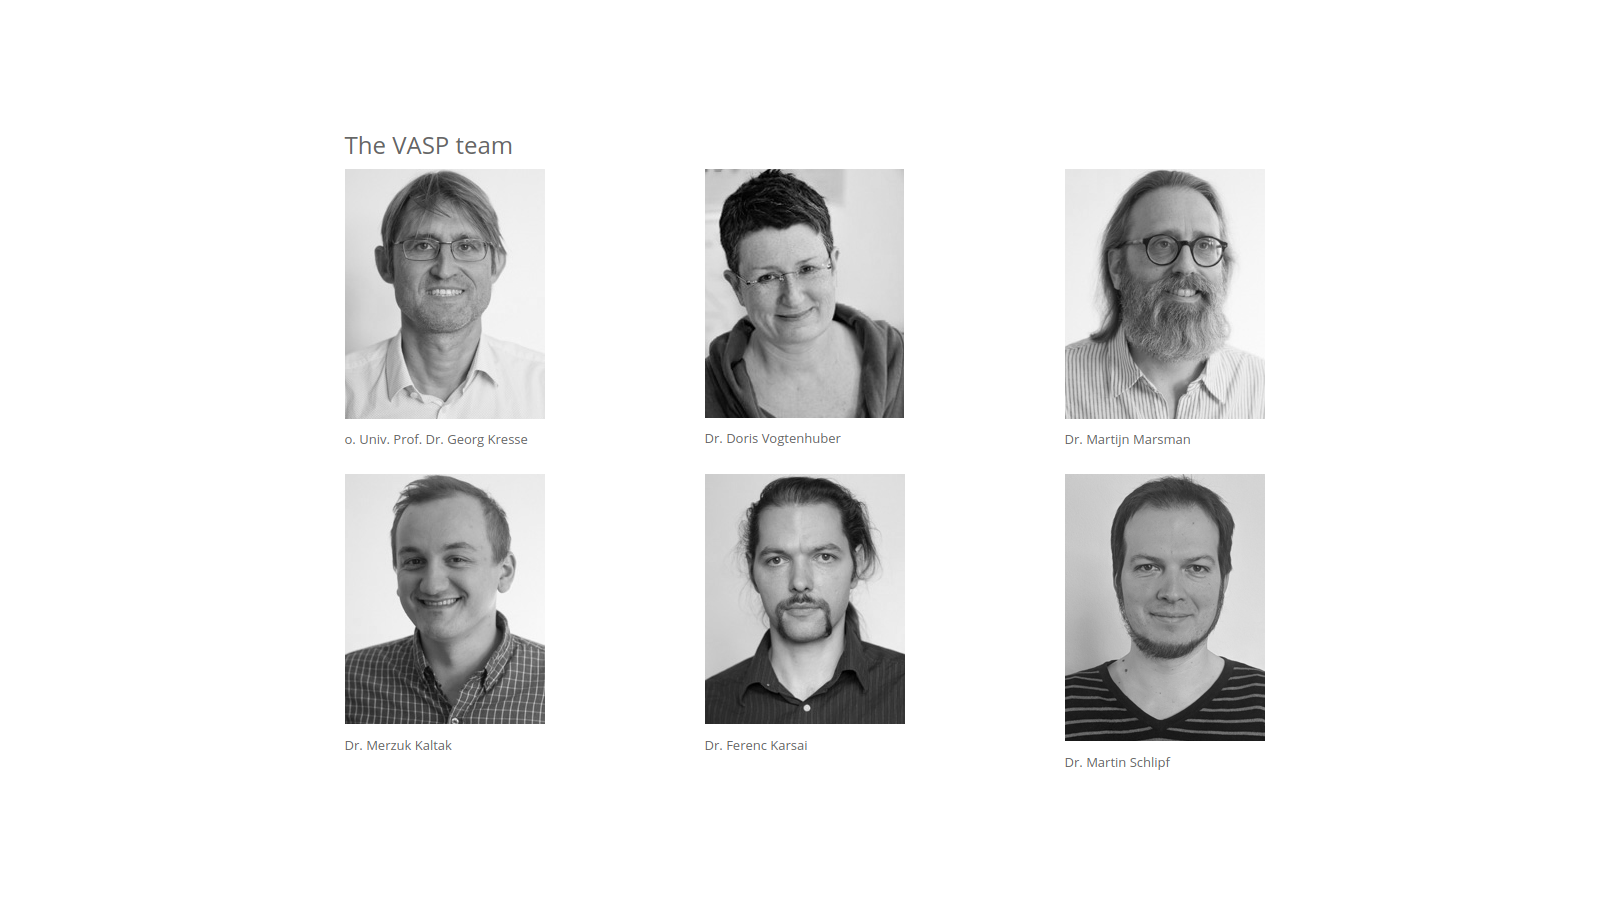
\includegraphics[height=2.70in,width=4.05in,viewport=330 130 1280 770,clip]{Figures/VASP_team.png}
\caption{\tiny \textrm{The development team of VASP.}}%(与文献\cite{EPJB33-47_2003}图1对比)
\label{VASP_team}
\end{figure}
}

\frame
{
	\frametitle{双网格技术}
\begin{figure}[h!]
	\vspace{-0.2in}
\centering
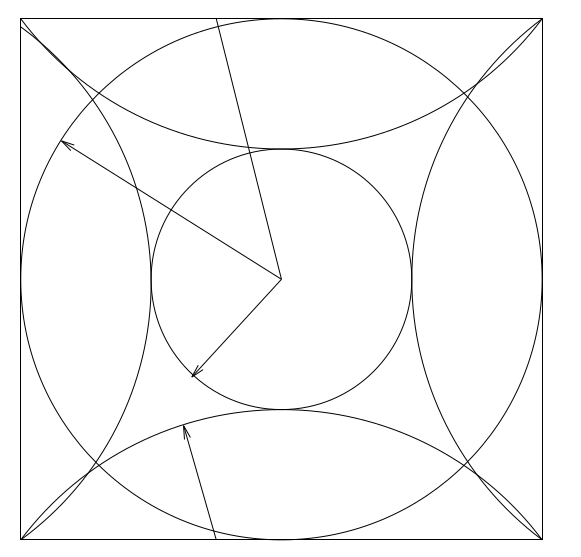
\includegraphics[height=2.3in,width=2.3in,viewport=0 0 420 420,clip]{Figures/VASP_G_max.png}
\caption{\fontsize{5.2pt}{3.9pt}\selectfont{\textrm{The small sphere contains all plane waves included in the basis set $\vec G<\vec G_\mathrm{cut}$. The charge density contains components up to $2\vec G$ cut (second sphere), and the acceleration a components up to $3\vec G$ cut , which are reflected in (third sphere) because of the finite size of the FFT-mesh. Nevertheless the components a $\vec G$ with $|\vec G|<\vec G$ cut are correct i.e. the small sphere does not intersect with the third large sphere.}}}%(与文献\cite{EPJB33-47_2003}图1对比)
\label{VASP_G_max}
\end{figure} 
}

\frame
{
	\frametitle{双网格技术}
\begin{figure}[h!]
	\vspace{-0.15in}
\centering
%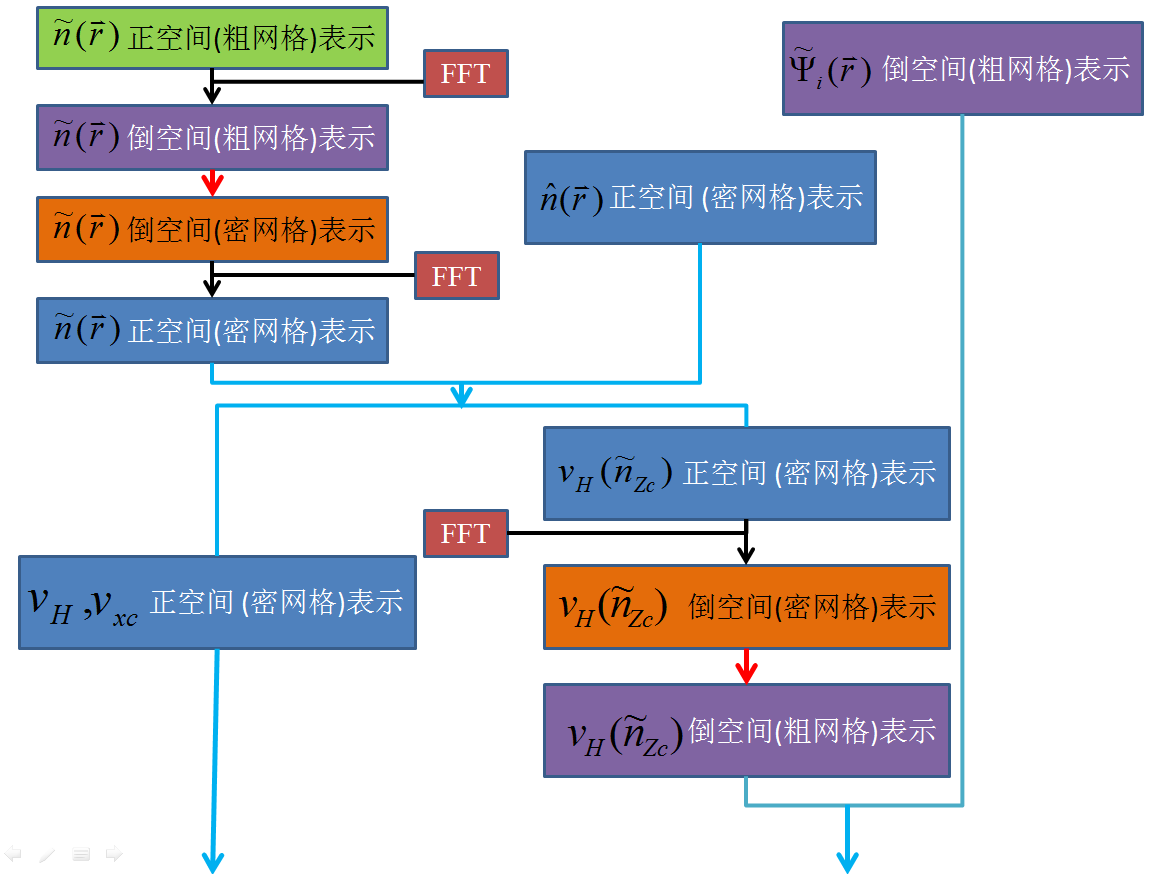
\includegraphics[height=2.7in,width=4.0in,viewport=0 0 1180 875,clip]{Figures/dual_grid.png}
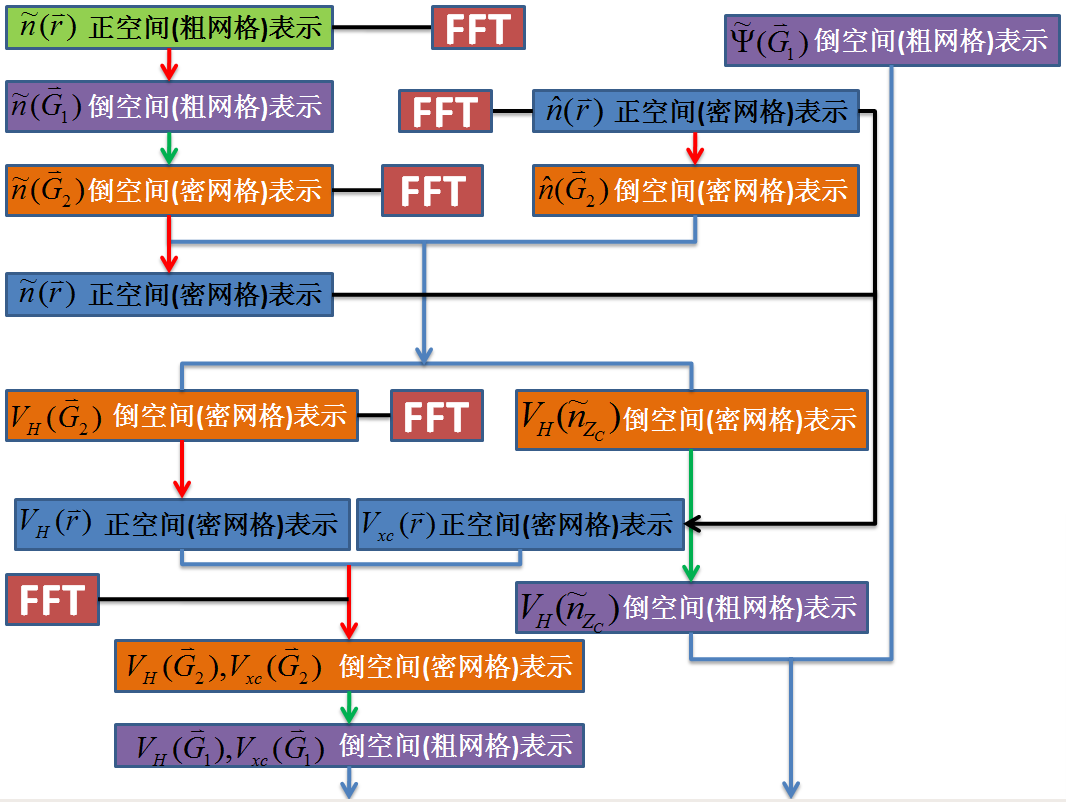
\includegraphics[height=2.75in,width=4.0in,viewport=0 0 800 600,clip]{Figures/dual_grid-2.png}
\caption{\tiny \textrm{The Schematic description of the dual grid technique.}}%(与文献\cite{EPJB33-47_2003}图1对比)
\label{PAW_dualgrid}
\end{figure} 
}

\frame
{
	\frametitle{\textrm{VASP}的平面波数目和内存估计}
	总的平面波数目计算公式
	\begin{displaymath}
		\begin{aligned}
			N_{\mathrm{PW}}=&\dfrac{4\pi}3\bigg(\dfrac{\vec G_{\mathrm{max}}\cdot\vec L}{2\pi}\bigg)^3\times\textcolor{blue}{1.1}\\
			=&\dfrac{4\pi}3\bigg(\sqrt{\dfrac{E_{\mathrm{cut}}}{\mathrm{RyToeV}}}\bigg)^3\times\dfrac{V_{\Omega}}{\mathrm{(a.u.To}\mbox{\textrm{\AA)}}^3}\times\dfrac1{8\pi^3}\times1.1
		\end{aligned}
	\end{displaymath}
	{\tiny 其中\textrm{RyToeV}是单位换算常数\textrm{13.605826};~\textrm{a.u.To\AA}是单位换算常数\textrm{0.529177249}}\\
	\begin{itemize}
		\item {\fontsize{9.2pt}{6.2pt}\selectfont{\textrm{VASP}要求的基本(预保留)内存为\textrm{30M}}}
		\item {\fontsize{9.2pt}{6.2pt}\selectfont{当体系规模较大时,波函数部分是内存消耗的最主要部分,其计算公式为\\
			\textcolor{red}{平面波部分}(单位\textrm{Byte})
			\begin{displaymath}
				16.0\times N_{\mathrm{PW}}\times N_{\mathrm{Band}}\times N_{\vec k\mathrm{pt}}\times N_{\mathrm{spin}}
			\end{displaymath}
			{\tiny 式中\textcolor{blue}{16}是双精度浮点数的内存}\\
			\textcolor{red}{局域波函数部分}
			\begin{displaymath}
				16.0\times N_{\mathrm{local}}\times N_{\mathrm{Band}}\times N_{\vec k\mathrm{pt}}\times N_{\mathrm{spin}}
			\end{displaymath}}}
	\end{itemize}
}

\frame
{
	\frametitle{\textrm{VASP}的平面波数目和内存估计}
	\begin{itemize}
		\item 非局域项投影函数计算分配的内存
		\item \textrm{FFT}变换分配内存
		\item 径向网格点分布分配内存
		\item 单中心在位项计算分配内存
	\end{itemize}
	并行计算时,如果节点数为$N_{\mathrm{node}}$,每个节点的核数$N_{\mathrm{core/node}}$,则平面波数目分配估算
	\begin{displaymath}
		\bar{N}_{\mathrm{PW/core}}=\dfrac{N_{\mathrm{PW}}}{N_{\mathrm{node}}\times N_{\mathrm{core/node}}}
	\end{displaymath}

	相应地,波函数的平面波部分所需的内存估计
				\begin{displaymath}
					16.0\times \textcolor{blue}{\min(N_{\mathrm{PW/core}})\times N_{\mathrm{node}}} \times N_{\mathrm{Band}}\times N_{\vec k\mathrm{pt}}\times N_{\mathrm{spin}}
				\end{displaymath}
}

\frame
{
	\frametitle{\textrm{VASP}的优化与迭代收敛}
	\textrm{VASP}计算中,资源消耗的主要部分是求解\textrm{Kohn-Sham}方程,即偏微分方程\textrm{(Partial Differential Equations,~PDE)}的自洽迭代, 迭代过程主要包括
	\begin{itemize}
		\item 矩阵的迭代对角化
		\item 电荷密度的自洽迭代
	\end{itemize}

	\vskip 10pt
	\textrm{VASP}的计算高效得益于求解过程中中应用了多种经典优化算法,保证了迭代计算的快速收敛
	\begin{itemize} 
		\item 拟牛顿法\textrm{(Quasi-Newton method)}
		\item 共轭梯度法\textrm{(Conjugate Gradients method, CG)}
		\item 残差最小化\textrm{(RMM-DIIS)}方法
	\end{itemize}
}

\subsection{经典数值优化算法概要}
\frame
{
	\frametitle{非线性方程的\rm{Newton~}法求根}
	\textcolor{blue}{不管哪一种数值算法,其设计原理都是将复杂转化为简单的重复,或者说,通过简单的重复生成复杂}:\\
	\textcolor{red}{在算法设计和算法实现过程中,重复就是力量}\\
迭代算法设计:~\textcolor{purple}{“速度”\textrm{vs}“稳定”}
\begin{figure}[h!]
\centering
\animategraphics[autoplay, loop, height=2.0in]{1}{Figures/OP_Newton_}{0}{17}
\label{Equation_Newon}
\end{figure}
}

\frame
{
	\frametitle{迭代优化基本思想}
	对于给定函数$f$,在极值点,函数的梯度满足
	\begin{displaymath}
		\nabla f=0
	\end{displaymath}
	可将函数极值问题转化成方程求根问题
\begin{figure}[h!]
\centering
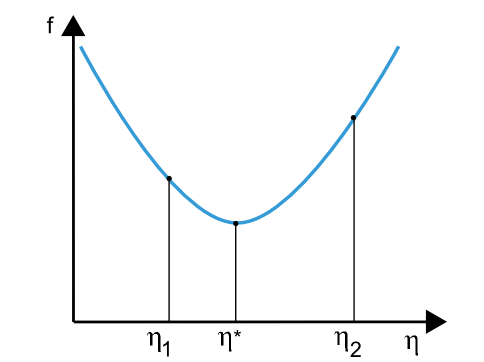
\includegraphics[height=1.68in,width=1.95in,viewport=30 0 450 360,clip]{Figures/OP_mini-1.png}
\hskip 0.05in
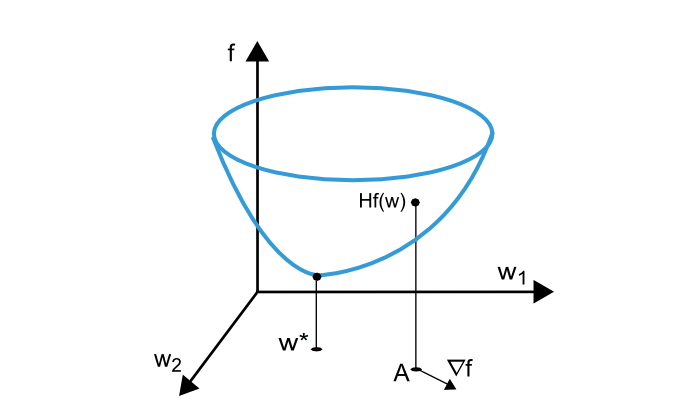
\includegraphics[height=1.68in,width=1.95in,viewport=150 20 560 390,clip]{Figures/OP_mini-2.png}
\label{OP_mini}
\end{figure}
}

\frame
{
	\frametitle{\textrm{Method of steepest descent}}
	对于函数$f(\mathbf{x}_0)$当前位置$\mathbf{x}_0$的负梯度方向$\mathbf{g}_0$满足
	\begin{displaymath}
		\mathbf{g}_0=-\nabla f(\mathbf{x}_0)
	\end{displaymath}
	用$\mathbf{g}_0$方向作为搜索方向,
	\begin{displaymath}
		\mathbf{x}=\mathbf{x}_0+\lambda\mathbf{g}_0,\qquad \lambda>0
	\end{displaymath}
	因为负的梯度方向为当前位置的最快下降方向,所以被称为“\textcolor{blue}{最陡下降法}”\\
	对函数$f$最小化参数$\lambda$,可确定下一步$\mathbf{x}_1$,可有
	\begin{displaymath}
		\dfrac{\mathrm{d}}{\mathrm{d}\lambda}f(\mathbf{x}_0+\lambda\mathbf{g})_0=\mathbf{g}_0\cdot\nabla f(\mathbf{x}_1)=\mathbf{g}_0\cdot\mathbf{g}_1=0
	\end{displaymath}
	因此\textcolor{red}{最速下降法最近邻两步的梯度彼此相互垂直}\\
	\textcolor{purple}{最陡下降法的收敛:~\\靠近极小值时收敛速度减慢,越接近目标,步长越小,前进越慢}
}

\frame
{
	\frametitle{\textrm{Newton-Raphson Method}}
	\textrm{Newton Method}是一种在实数和复数域上近似解方程的方法。\\
	思想:~\textcolor{blue}{用函数的\textrm{Taylor}级数的前几项来寻找方程$f(x)=0$的根}\\
	由\textrm{Newton}迭代公式有
	\begin{displaymath}
		x_{n+1}=x_n-\dfrac{f(x_n)}{f^{\prime}(x_n)}
	\end{displaymath}
	用\textrm{Taylor}级数在$a$附近展开$f(x)$
	\begin{displaymath}
		f(x)=\sum_{n=0}^{\infty}\dfrac{f^{(n)}(a)}{n!}(x-a)^n
	\end{displaymath}
	如果只取其前两项逼近$f(x)$,可有
	\begin{displaymath}
		f(x)=f(a)+f^{(1)}(a)(x-a)
	\end{displaymath}
	不难看出$x=a-\frac{f(a)}{f^{(1)}(a)}$时,有$f(x)=0$
}

\frame
{
	\frametitle{\textrm{Newton-Raphson Method}}
	对于函数求极值问题(函数的导数为零),就转换成
	\begin{displaymath}
		x_{n+1}=x_{n}-\dfrac{f^{(1)}(x_n)}{f^{(2)}(x_n)}
	\end{displaymath}
	对高维函数,一阶导数是梯度,二阶导数是\textcolor{blue}{\textrm{Hessian}矩阵}\\$\mathbf{H}f(\mathbf{x})=[\frac{\partial^2f}{\partial x_i\partial x_j}]_{n\times n}$,有
	\begin{displaymath}
		x_{n+1}=x_n-\alpha[\mathbf{H}f(x_n)]^{-1}\nabla f(x_n)\quad n\geqslant0
	\end{displaymath}
	这里$\alpha$是可调参数%,$\mathbf{H}$是\textrm{Hessian}矩阵

	\begin{itemize}
		\item 最陡下降法是用一个平面去拟合当前位置的局部曲面
		\item \textrm{Newton}法是用一个二次曲面拟合当前位置的局部曲面
	\end{itemize}
通常情况下,二次曲面的拟合会比平面更好,所以牛顿法选择的路径会更符合真实的最优下降路径(收敛更快)

\textcolor{magenta}{\textrm{Newton}法的缺点:~\textrm{Hessian}矩阵求逆的计算成本和复杂度较高}
}

\frame
{
	\frametitle{\textrm{Quasi-Newton Method}}
	\textrm{Newton}法收敛速度快,但计算过程中需计算\textrm{Hessian}矩阵(而且无法保证正定),因此有了\textrm{Quasi-Newton}方法\\
	思想:~\textcolor{blue}{构造可以近似\textrm{Hessian}矩阵(或逆)的正定对称阵}
		{\fontsize{7.2pt}{4.2pt}\selectfont{
	\begin{displaymath}
		f(\mathbf{x})\approx f(\mathbf{x}_{k+1})+\nabla f(\mathbf{x}_{k+1})(\mathbf{x}-\mathbf{x}_{k+1})+\dfrac12(\mathbf{x}-\mathbf{x}_{k+1})\nabla^2f(\mathbf{x}_{k+1})(\mathbf{x}-\mathbf{x}_{k+1})
	\end{displaymath}
	两边作用梯度算符$\nabla$
	\begin{displaymath}
		\nabla f(\mathbf{x})\approx\nabla f(\mathbf{x}_{k+1})+\mathbf{H}_{k+1}(\mathbf{x}-\mathbf{x}_{k+1})
	\end{displaymath}
	当$\mathbf{x}=\mathbf{x}_k$有
	\begin{displaymath}
		\mathbf{g}_{k+1}-\mathbf{g}_k\approx\mathbf{H}_{k+1}(\mathbf{x}-\mathbf{x}_k)
	\end{displaymath}
令
\begin{displaymath}
	\mathbf{s}_k=\mathbf{x}_{k+1}-\mathbf{x}_k\quad\mathbf{y}_k=\mathbf{g}_{k+1}-\mathbf{g}_k
\end{displaymath}
有
\begin{displaymath}
	\mathbf{y}_k\approx\mathbf{H}_{k+1}\cdot\mathbf{s}_k\quad\mbox{或}\quad\mathbf{s}_k\approx\mathbf{H}_{k+1}^{-1}\mathbf{y}_{k}
\end{displaymath}}}
{\fontsize{9.2pt}{4.2pt}\selectfont{\textcolor{purple}{\textrm{Quasi-Newton}法:~靠近极小值时收敛速快;~初值选择不好,易不收敛}}}
}

\frame
{
	\frametitle{共轭梯度的``轭''}
\begin{figure}[h!]
\centering
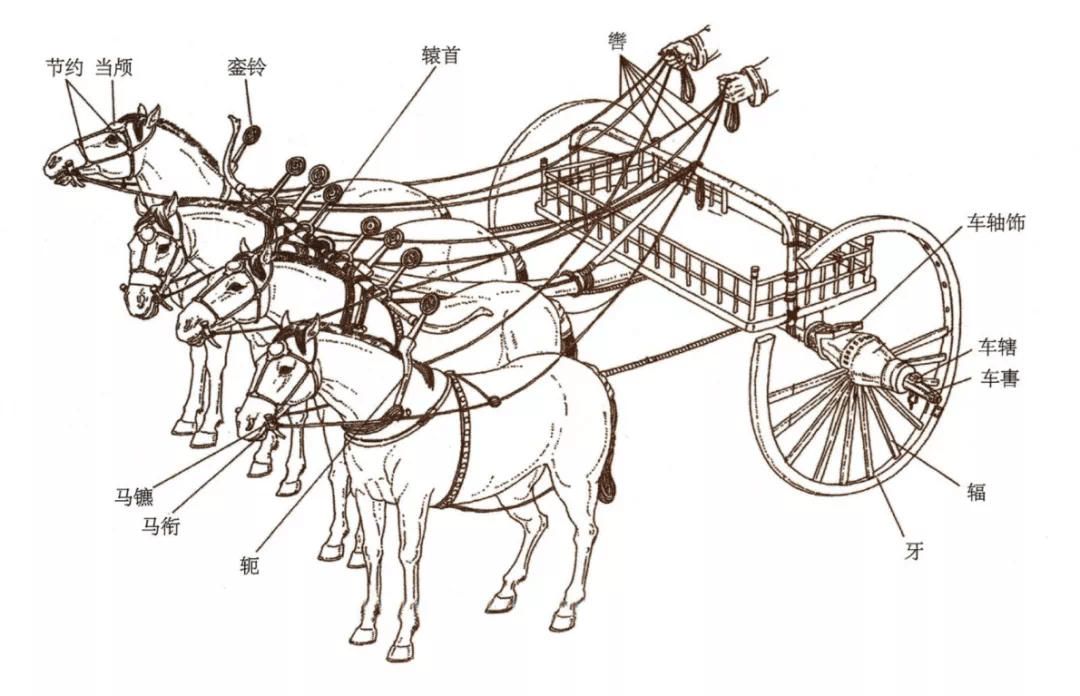
\includegraphics[height=2.5in,width=4.0in,viewport=0 0 1050 680,clip]{Figures/Yoke_1.png}
\label{Horse_Yoke}
%\caption{\tiny \textrm{Schematic illustration of minimization of a function in two dimensions. The steps 1,2,3,$\cdots$ denote the steepest descent steps and the point $2^{\ast}$ denote the conjugate gradient path that reaches the exact solution after two steps if the functional is quadratic.}}%(与文献\cite{EPJB33-47_2003}图1对比)
\end{figure}
}

\frame
{
	\frametitle{共轭的含义}
\begin{minipage}{0.63\textwidth}
\begin{figure}[h!]
\vskip -23pt
\centering
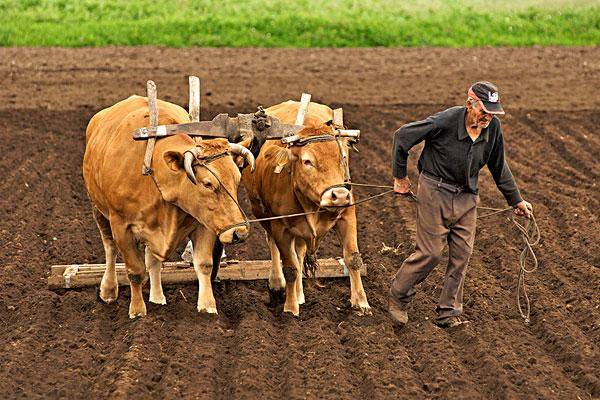
\includegraphics[height=1.6in,width=2.2in,viewport=0 0 600 490,clip]{Figures/Bi-Yoke_1.jpg}
\vskip 2pt
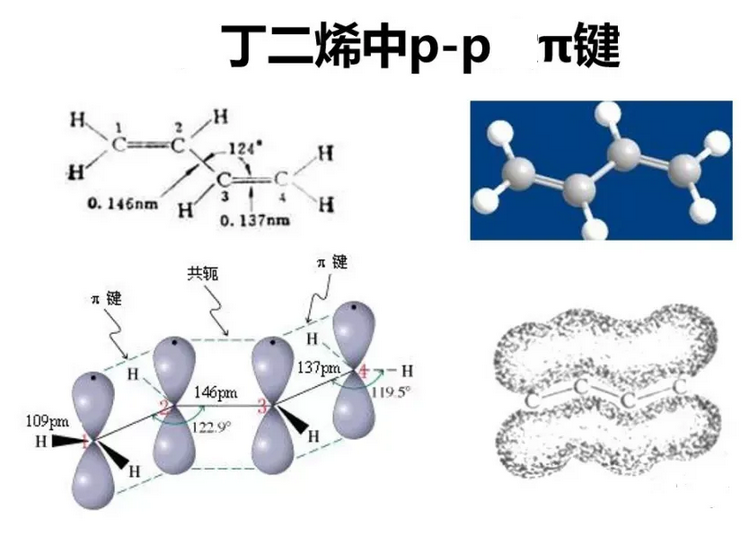
\includegraphics[height=1.5in,width=2.2in,viewport=0 0 750 530,clip]{Figures/Conjugate_Pi-bond.png}
\label{Conjugate_1}
%\caption{\tiny \textrm{Schematic illustration of minimization of a function in two dimensions. The steps 1,2,3,$\cdots$ denote the steepest descent steps and the point $2^{\ast}$ denote the conjugate gradient path that reaches the exact solution after two steps if the functional is quadratic.}}%(与文献\cite{EPJB33-47_2003}图1对比)
\end{figure}
\end{minipage}
\begin{minipage}{0.35\textwidth}
\begin{figure}[h!]
\centering
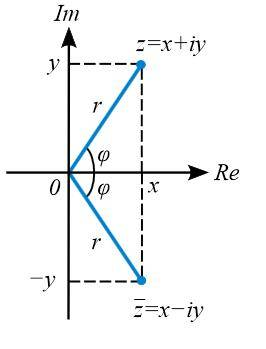
\includegraphics[height=2.2in,width=1.5in,viewport=0 0 250 390,clip]{Figures/Conjugate_complex.jpg}
\label{Conjugate_2}
%\caption{\tiny \textrm{Schematic illustration of minimization of a function in two dimensions. The steps 1,2,3,$\cdots$ denote the steepest descent steps and the point $2^{\ast}$ denote the conjugate gradient path that reaches the exact solution after two steps if the functional is quadratic.}}%(与文献\cite{EPJB33-47_2003}图1对比)
\end{figure}
\end{minipage}
}

\frame
{
	\frametitle{\textrm{Conjugate gradient}}
	假设函数在接近极值附件,近似有\textcolor{magenta}{二次函数}的形式
	\begin{displaymath}
		f(\mathbf{x})=f_0+\frac12\mathbf{x}\cdot\mathbf{H}{\mathbf{x}}+\cdots
	\end{displaymath}
	其中$\mathbf{H}$是\textcolor{blue}{\textrm{Hessian}矩阵}%,定义为
%	\begin{displaymath}
%		H_{ij}=\dfrac{\partial^2f(\mathbf{x})}{\partial x_i\partial x_j}
%	\end{displaymath}
	当$f$的偏导连续,则$\mathbf{H}$是对称矩阵,并且一般要求$\mathbf{H}$是正定的。相应的梯度表示为
	\begin{displaymath}
		\mathbf{g}=\nabla f(\mathbf{x})=-\dfrac{\partial f}{\partial\mathbf{x}}=-\mathbf{H}\cdot\mathbf{x}
	\end{displaymath}
	\vskip 20pt
	设从点$\mathbf{x}_i$出发沿方向$\mathbf{h}_i$(\textcolor{blue}{不再限于梯度$\mathbf{g}_i$方向}),前进到点$\mathbf{x}_{i+1}$,根据最小化要求
	\begin{displaymath}
		\mathbf{h}_i\cdot\nabla f(\mathbf{x}_{i+1})=0
	\end{displaymath}
	为确定$\mathbf{x_{i+1}}$点的继续前进方向$\mathbf{h}_{i+1}$,设$\mathbf{x}_{i+1}$可由$\mathbf{x}_i+\lambda\mathbf{h}_{i+1}$得到,因此$\mathbf{x}_{i+1}$的梯度
	\begin{displaymath}
		\mathbf{g}_{i+1}=\nabla f(\mathbf{x}_{i+1})=-\mathbf{H}\mathbf{x}_{i+1}=-\mathbf{H}(\mathbf{x}_{i}+\lambda\mathbf{h}_{i+1})
	\end{displaymath}
}

\frame
{
	\frametitle{\textrm{Conjugate gradient}}
	与方向$\mathbf{h}_i$相比,梯度的改变为
	\begin{displaymath}
		\Delta\mathbf{g}=-\lambda\mathbf{H}\mathbf{h}_{i+1}
	\end{displaymath}

	根据最小化要求,梯度的改变与$\mathbf{h}_i$方向正交
	\begin{displaymath}
		\mathbf{h}_i\cdot\mathbf{H}\cdot\mathbf{h}_{i+1}=0
	\end{displaymath}
	共轭梯度法算法:对于给定函数
	\begin{itemize}
		\item 已知初值$\mathbf{x}_0$和梯度$\mathbf{g}_0$,取初始方向$\mathbf{h_0}=\mathbf{g}_0$(\textcolor{blue}{最陡下降})
		\item 根据递推关系确定
			\begin{displaymath}
				\begin{aligned}
					\mathbf{g}_{i_+1}=&\mathbf{g}_{i_+1}-\lambda_i\mathbf{H}\mathbf{h}_{i}\qquad \lambda_i=\dfrac{\mathbf{g}_i\cdot\mathbf{g}_i}{\mathbf{g}_i\cdot\mathbf{H}\mathbf{h}_i}\\	
					\mathbf{h}_{i_+1}=&\mathbf{g}_{i_+1}+\gamma_i\mathbf{h}_{i}\qquad \gamma_i=-\dfrac{\mathbf{g}_{i+1}\cdot\mathbf{H}\mathbf{h}_i}{\mathbf{h}_i\cdot\mathbf{H}\mathbf{h}_i}\\	
					\mathbf{x}_{i_+1}=&\mathbf{x}_{i}+\lambda_i\mathbf{h}_{i}
				\end{aligned}
			\end{displaymath}
	\end{itemize}
	\textcolor{purple}{共轭梯度法的收敛:~步收敛性,稳定性高,不需要任何外来参数}
}

\frame
{
	\frametitle{最陡下降与共轭梯度}
\begin{figure}[h!]
\centering
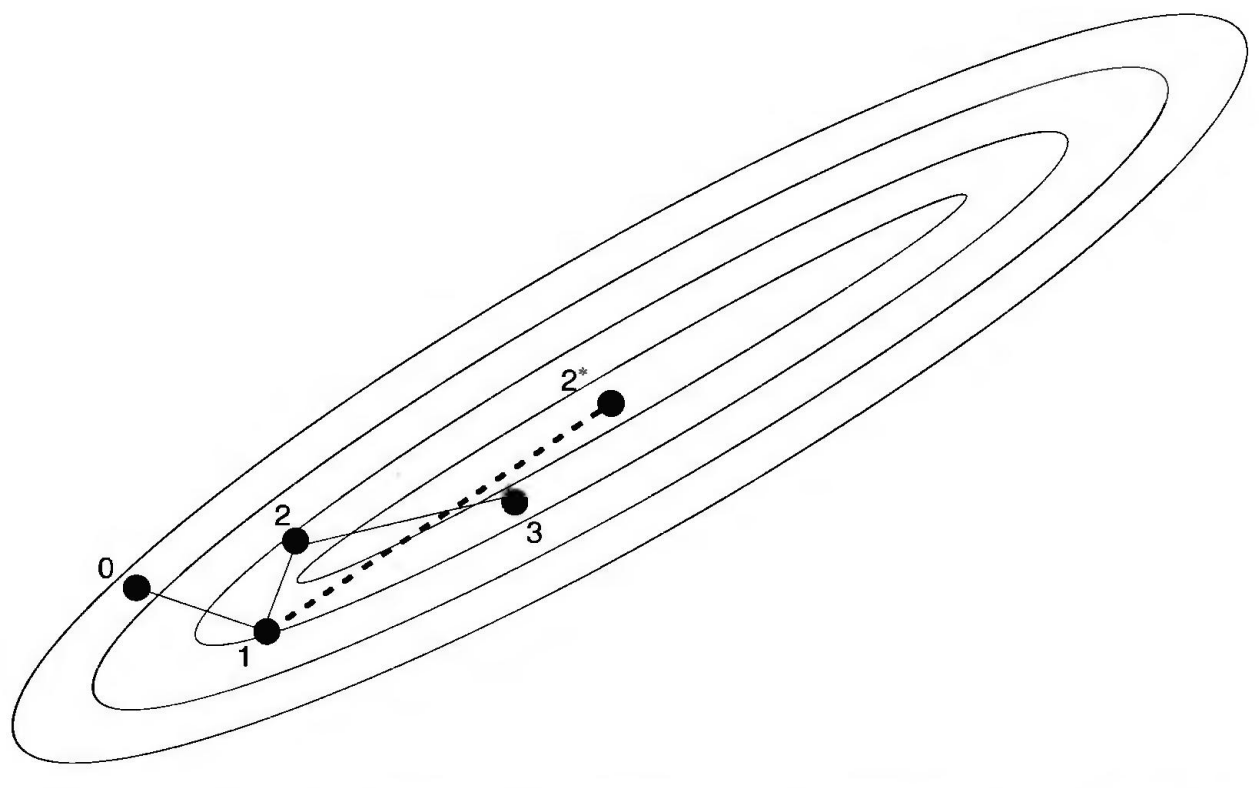
\includegraphics[height=2.0in,width=3.5in,viewport=0 0 950 590,clip]{Figures/OP_descent_CG.png}
\label{decent_CG}
\caption{\tiny \textrm{Schematic illustration of minimization of a function in two dimensions. The steps 1,2,3,~$\cdots$ denote the steepest descent steps and the point - \!- \!- \!- \!- \!- denote the conjugate gradient path that reaches the exact solution after two steps if the functional is quadratic.}}%(与文献\cite{EPJB33-47_2003}图1对比)
\end{figure}
}

\frame
{
	\frametitle{\textrm{Fixed Point}}
	求解方程
	\begin{displaymath}
		f(\mathbf{x})=\mathbf{x}
	\end{displaymath}
	$\mathbf{x}$是函数$f(\mathbf{x})$的\textcolor{red}{不动点}
	
	对这类问题的求解,可以利用迭代关系
	\begin{displaymath}
		\mathbf{x}_{i+1}=f(\mathbf{x}_i)\qquad (i=1,2,3,\cdots)
	\end{displaymath}
	这称为\textcolor{blue}{不动点迭代法}

	{\fontsize{6.2pt}{4.2pt}\selectfont{例如求解方程
	\begin{displaymath}
%		\begin{aligned}
			\lg(10+x)~=~x%\\
			\Longrightarrow	\textcolor{blue}{x\approx 1.04309063}
%		\end{aligned}
		\end{displaymath}}}
\begin{minipage}[b]{0.35\textwidth}
		{\fontsize{3.2pt}{1.2pt}\selectfont{
	\begin{displaymath}
	\vspace{-0.11in}
		\begin{aligned}
			x_0&=1 %~\Longrightarrow 
			\\\lg(10+1)&=1.041392685\\
x_1 &=1.041392685 %~\Longrightarrow 
\\\lg(10+1.041392685)&=1.0430238558\\
x_2 &=1.043023856 %~\Longrightarrow 
\\\lg(10+1.043023856)&=1.0430880104\\
x_3 &=1.043088010 %~\Longrightarrow 
\\\lg(10+1.043088010)&=1.0443090533\\
x_4 &=1.043090533 %~\Longrightarrow 
\\\lg(10+1.043090533)&=1.04430906326\\
x_4 &=1.0430906326 %~\Longrightarrow 
\\\lg(10+1.0430906326)&=1.04430906365\\
x_5 &=1.0430906365 %~\Longrightarrow 
\\\lg(10+1.0430906365)&=1.04430906366\\
x_6 &=1.0430906366 %~\Longrightarrow 
\\\lg(10+1.0430906366)&=1.04430906366
		\end{aligned}
	\end{displaymath}}}
\end{minipage}
\hfill
\begin{minipage}[b]{0.62\textwidth}
\begin{figure}[h!]
	\vspace{-0.21in}
\centering
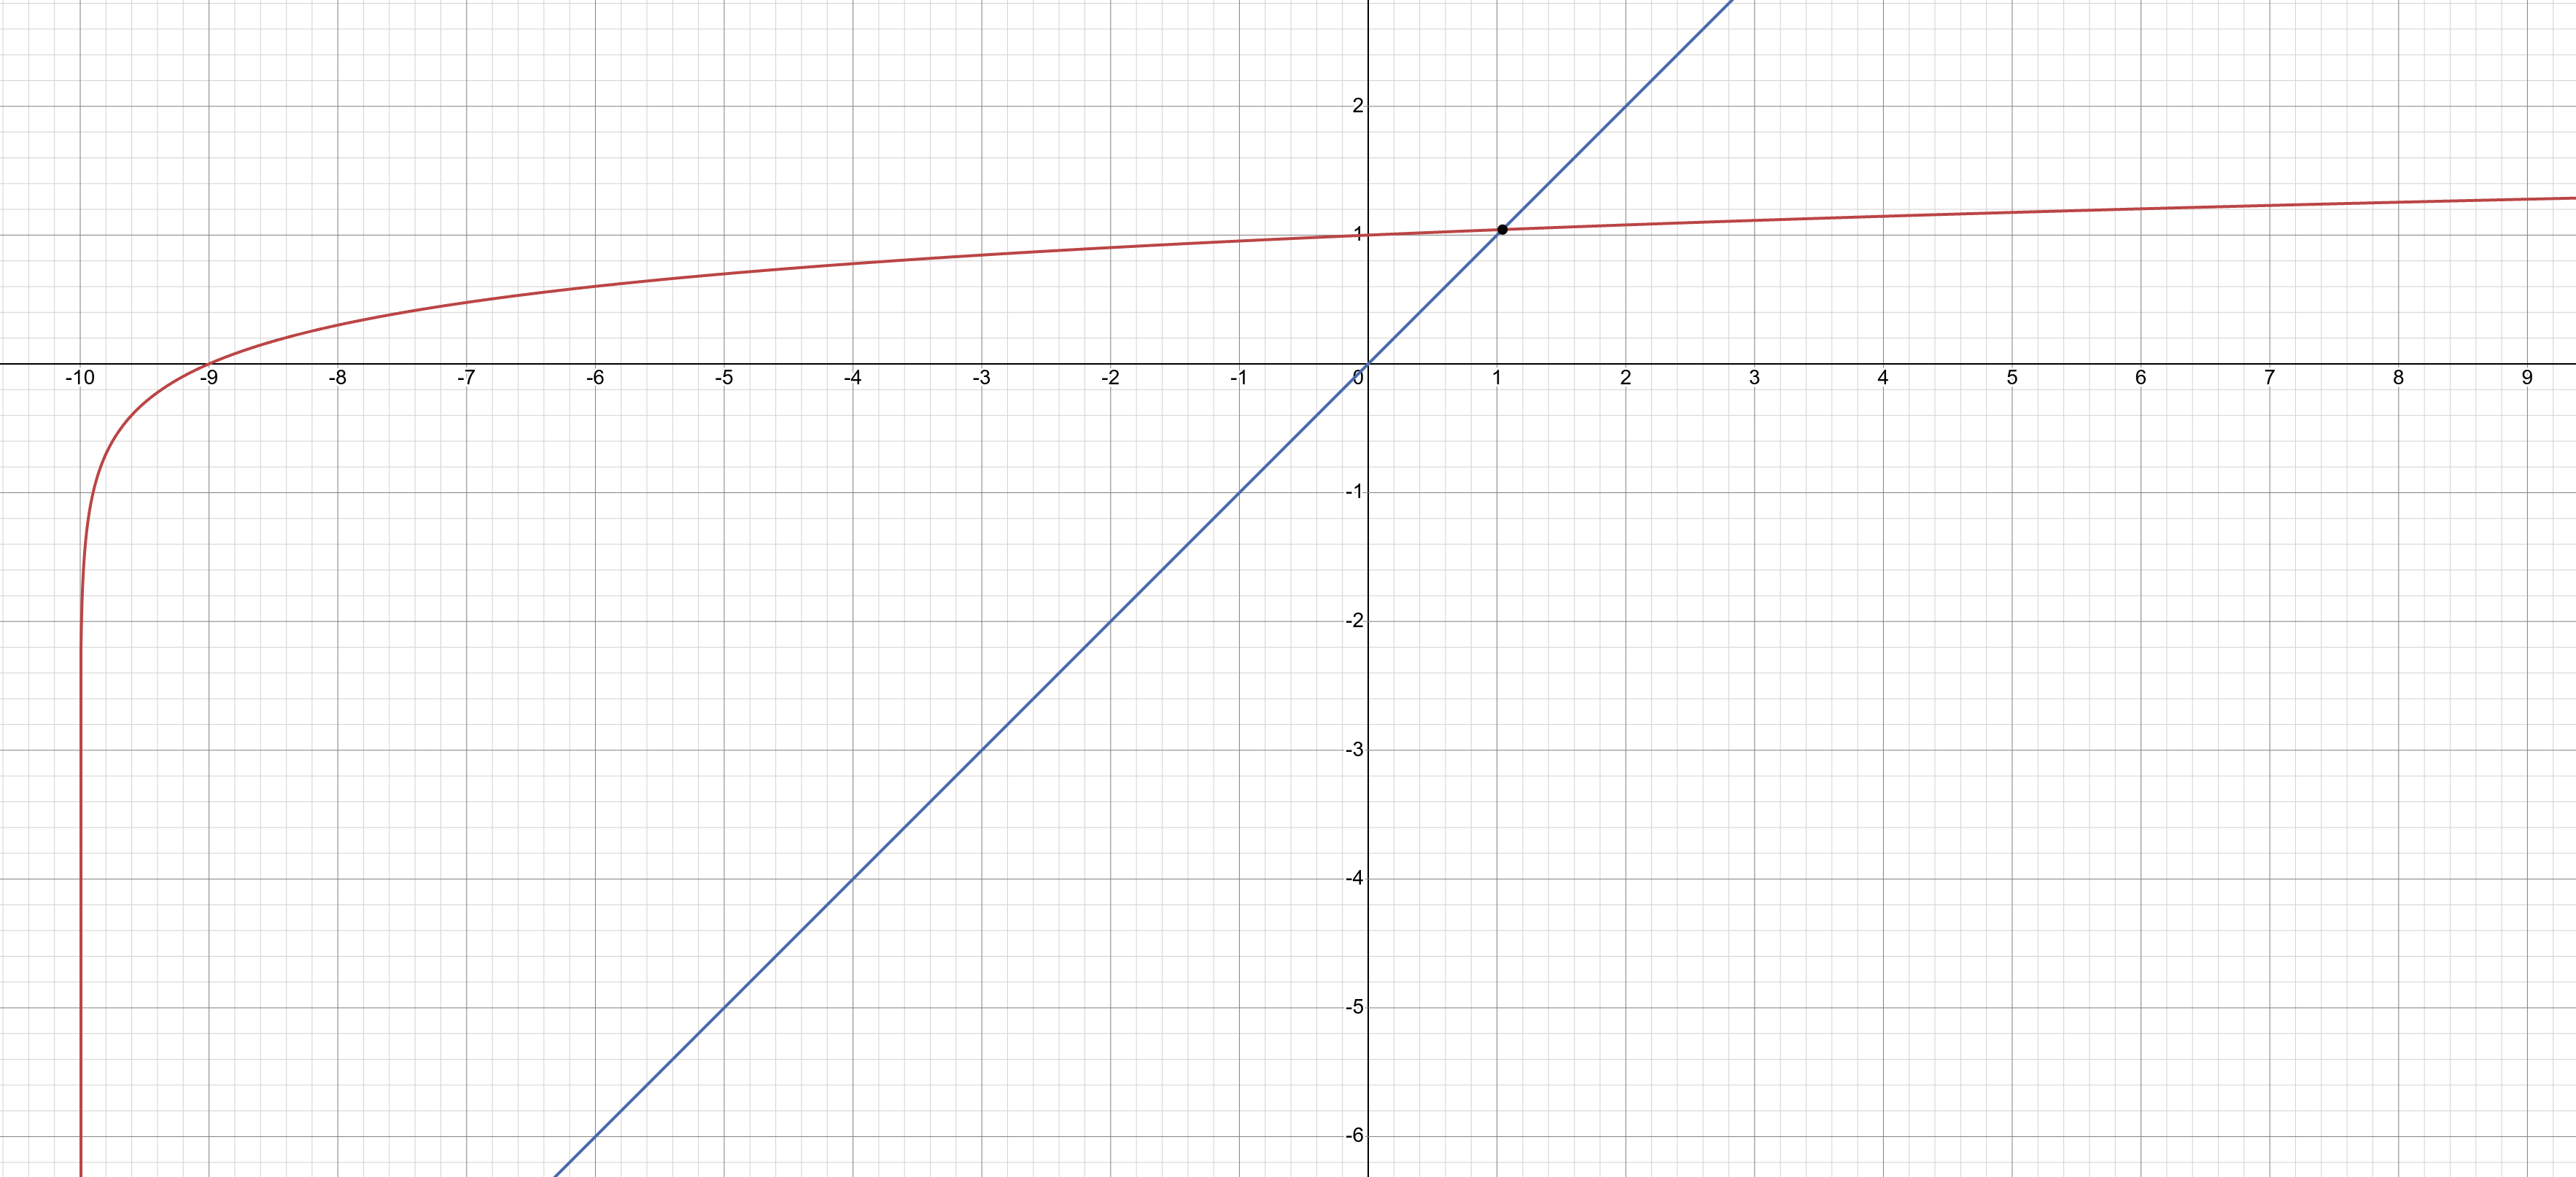
\includegraphics[height=1.3in,width=2.0in,viewport=0 0 2500 1600,clip]{Figures/solve_lg10.png}
%\caption{\tiny \textrm{The comparison of parallel scaling for ABINIT vs VASP.}}%(与文献\cite{EPJB33-47_2003}图1对比)
\label{solution-log_10}
\end{figure}
\end{minipage}
}

\frame
{
	\frametitle{\textrm{Residue minimization Methods}}
不动点迭代的主要问题是对初猜的依赖,很可能不收敛或线性收敛(收敛缓慢),一种求解策略是定义残量
	\begin{displaymath}
		R[\mathbf{x}]=f(\mathbf{x})-\mathbf{x}
	\end{displaymath}
	最小化残量的模$|R[\mathbf{x}]|$,特别是当残量$R[\mathbf{x}]$近似是$\mathbf{x}$的线性函数,可有\textcolor{purple}{\textrm{Jacobian}矩阵}
	\begin{displaymath}
		\mathbf{J}\equiv\dfrac{\delta R[\mathbf{x}]}{\delta\mathbf{x}}
	\end{displaymath}
	然后可以用\textrm{Quasi-Newton}方法最小化残量\\具体地可通过迭代关系求解原方程的解
	\begin{displaymath}
		\mathbf{x}_{i+1}=\mathbf{x}_{i}-\mathbf{J}^{-1}R[\mathbf{x}_{i}]
	\end{displaymath}
		但是一般来说\textrm{Jacobian}矩阵很可能未知(或者很难求逆),只有另图别策(在\textrm{Krylov}子空间中迭代求解),一般常用的方法有
		\begin{itemize}
			\item 迭代子空间求逆(\textrm{Discret Inversion in the Iterative Subspace,~DIIS})
			\item \textrm{Anderson}加速或\textrm{Anderson}混合
		\end{itemize}
}
	
\frame
{
	\frametitle{\textrm{Pulay DIIS full-subspace Metheod}}
	{\fontsize{7.2pt}{1.2pt}\selectfont{\textrm{DIIS}是\textrm{Pulay}引入的,俗称的\textcolor{blue}{\textrm{Pulay}混合}\footnote{\fontsize{5.2pt}{1.2pt}\selectfont{一般地说,\textrm{DIIS}是通用的不动点迭代的加速收敛方法;~对于线性问题,\textrm{DIIS}等价于\textrm{GMRES}方法}}}}\\
	{\fontsize{5.2pt}{1.2pt}\selectfont{其思想是:~对迭代逼近的矢量$\mathbf{x}_{i}$,可通过将之前得到的所有矢量$\mathbf{x}$线性组合得到,组合系数则由对其残矢最小化确定。概要如下\\
	在由$\mathbf{x}_i$构成的完全\textrm{Krylov}子空间内,有矢量
	\begin{displaymath}
		\mathbf{x}_{i+1}=\sum_{j=0}^{i}a_j\mathbf{x}_j=c_0\mathbf{x}_0+\sum_{j=1}^ic_j\delta\mathbf{x}_j
	\end{displaymath}
	若假设该矢量的残矢$R[\mathbf{x}_{i+1}]$与矢量$\mathbf{x}_{i+1}$满足相同的线性化要求
	\begin{displaymath}
		R[\mathbf{x}_{i+1}]=R[\sum_{j=0}^ia_j\mathbf{x}_j]=\sum_{j=0}^ia_jR[\mathbf{x}_j]
	\end{displaymath}
	通过最小化残矢的模
	\begin{displaymath}
		\langle R[\mathbf{x}_{i+1}]|R[\mathbf{x}_{i+1}]\rangle=\sum_{j,k}a_ja_kA_{j,k};A_{j,k}=\langle R[\mathbf{x}_j]|R[\mathbf{x}_k]\rangle
	\end{displaymath}
	即可确定矢量$\mathbf{x}_{i+1}$

	在电子结构计算中,残矢最小化的约束条件最常用的有
	\begin{itemize}
		\item 电子能带的本征矢正交
		\item 电荷密度混合时,电荷密度守恒,即$\sum\limits_{j=0}^i a_j=1$,可有\\\textcolor{blue}{$a_j=\sum\limits_jA_{j,i}^{-1}/\sum\limits_{j,k}a_ja_kA_{j,k}^{-1}=\sum\limits_jA_{j,i}^{-1}/\sum\limits_{j,k}A_{j,k}^{-1}$
%				\begin{displaymath}
%					\begin{aligned}
%						a_j=\sum\limits_jA_{j,i}^{-1}/\sum\limits_{j,k}&\underbrace{a_ja_k}A_{j,k}^{-1}\\
%						&\mbox{\textcolor{purple}{可略去}}
%					\end{aligned}
%				\end{displaymath}
		}
	\end{itemize}
}}
}

\frame
{
	\frametitle{\textrm{Broyden Jacobian update method}}
	最初的\textrm{Broyden}方法是\textcolor{magenta}{迭代过程中连续产生\textrm{Jacobian}逆阵的方案}
	{\fontsize{5.2pt}{1.2pt}\selectfont{
		\begin{itemize}
			\item 作为迭代起点,首先初猜合理的$\mathbf{J_0}^{-1}$(比如$\mathbf{J}_0^{-1}=\alpha\mathbf{I}$)
			\item 迭代开始的若干步内,保持$\mathbf{J}^{-1}$为初猜形式;~后续$\mathbf{J}^{-1}$再逐步更新:~
		因为$\mathbf{J}^{-1}$始终是近似的,有
				\begin{displaymath}
					\begin{aligned}
						\delta\mathbf{x}_i=&\mathbf{x}_i-\mathbf{x}_{i-1}=-\mathbf{J}_{i-1}^{-1}R_{i-1}\\
						\delta R_i=&R_i-R_{i-1}
					\end{aligned}
				\end{displaymath}
				因此要求每一步迭代更新的$\mathbf{J}_i^{-1}$满足
\begin{displaymath}
	0=\delta\mathbf{x}_i-\mathbf{J}_i^{-1}\delta R_i
\end{displaymath}
由此得到构成$M\times M$的$\mathbf{J}_i^{-1}$的$M$个方程
\item 最小化\textrm{Jacobian}逆阵的模变化
	\begin{displaymath}
		Q=||\mathbf{J}_{i}^{-1}-\mathbf{J}_{i}^{-1}||
	\end{displaymath}
	\textcolor{magenta}{\begin{displaymath}
			\mathbf{J}_i^{-1}=\mathbf{J}_{i-1}^{-1}\dfrac{(\delta\mathbf{x}_i-\mathbf{J}_i^{-1}\delta R_i)\delta R_i}{\langle\delta R_i|\delta R_i\rangle}
		\end{displaymath}}
		\end{itemize}
}}
	改进的\textrm{Broyden}方法与\textrm{DIIS}方法的结果类似,可以节约内存
	{\fontsize{5.2pt}{1.2pt}\selectfont{
	\begin{displaymath}
		Q^{\mathrm{modified}}=\sum_{j=1}^i w_j|\delta\mathbf{x}_j-\mathbf{J}_i^{-1}\delta R_j|^2+w_0||\mathbf{J}_i^{-1}-\mathbf{J}_0^{-1}||
	\end{displaymath}
	通过参数$w_j$筛选出迭代步中与之最密切关联的贡献
}}
}

\frame
{
	\frametitle{\textrm{Anderson acceleration}}
	\textrm{Donald~G.~Anderson}给出了加速不动点迭代的求解思路
	{\fontsize{7.2pt}{1.2pt}\selectfont{
	\begin{displaymath}
		\begin{aligned}
			\mathbf{x}_1=&f(\mathbf{x_0})\\
			\forall k=&1,2,\cdots\\
			&m_k=\min\{m,k\}\\
			&R_k=[R_{k-m_k},\cdots,R_k]\\
			&\alpha_k={\mathrm{argmin}}_{\alpha\in A_k}||R_k\alpha||_2,~\mbox{这里}A_k=\{\alpha=(\alpha_0,\alpha_1,\cdots,\alpha_{m_k})~\mbox{并满足}\sum\limits_{i=0}^n\alpha_i=1\}\\
			&\mathbf{x}_{k+1}=\sum_{i=0}^{m_k}(\alpha_k)_if_{k-m_k+i}
		\end{aligned}
	\end{displaymath}
}}
\begin{itemize}
	\item \textrm{Anderson}本质上是\textrm{Quasi-Newton}方法求解非线性方程(是割线方法的推广),也可以归入\textrm{Broyden}方法一类

	\item \textrm{Anderson}加速数学形式上可以看成\textrm{Generalized Minimal RESidual Method~(GMRES)}迭代推广到非线性方程求解,只是作了适当的截断
\end{itemize}
}

\frame
{
	\frametitle{\textrm{Anderson acceleration}}
	{\fontsize{6.2pt}{1.2pt}\selectfont{
	具体地,在迭代过程中,引入中间变量
	\begin{displaymath}
		\mathbf{x}_{i+1}^{\prime}=\alpha_k\mathbf{X}_k
	\end{displaymath}
	这里$\alpha_k$是组合系数$a_k\in A_k~$,~$\mathbf{X}_k=[\mathbf{x}_{k-m_k},\cdots, \mathbf{x}_k]$是含有最近$m_k+1$个矢量的矩阵\\
	选择合适的$\mathbf{x}_{k+1}^{\prime}$使得$||R(\mathbf{x}_{k+1}^{\prime})||$最小化

	因为$\alpha_k$的求和为1,有一阶近似
	\begin{displaymath}
		R(\mathbf{X}_k\alpha_k)=R\bigg(\sum_{i=0}^{m_k}(\alpha_k)_i\mathbf{x}_{k-m_k+i}\bigg)\approx\sum_{i=0}^{m_k}(\alpha_k)_iR(\mathbf{x}_{k-m_k+i})=R_k\alpha_k
	\end{displaymath}
	因此可以通过最小化$||R_k\alpha||_2$确定$\alpha$,进而确定$\mathbf{x}_{k+1}^{\prime}$
	
	考虑到$f(\mathbf{x})=\mathbf{x}$的精确解$\mathbf{x}^{\ast}$,因此$f(\mathbf{x}_{k+1}^{\prime})$可能比$\mathbf{x}_{k+1}^{\prime}$更接近$\mathbf{x}^{\ast}$,因此最终方程的解选为$\mathbf{x}_{k+1}=f(\mathbf{x}_{k+1}^{\prime})$而非$\mathbf{x}_{k+1}=\mathbf{x}_{k+1}^{\prime}$

类似地,因为$\alpha_k$的求和为1,有一阶近似
\begin{displaymath}
	f(\mathbf{x}_{k+1}^{\prime})=f\bigg(\sum_{i=0}^{m_k}(\alpha_k)_i\mathbf{x}_{k-m_k+i}\bigg)\approx\sum_{i=0}^{m_k}(\alpha_k)_if(\mathbf{x}_{k-m_k+i})=\sum_{i=0}^{m_k}(\alpha_k)_if_{k-m_k+i}
\end{displaymath}
最终确定方程的解为
\begin{displaymath}
	\mathbf{x}_{k+1}=\sum_{i=0}^{m_k}(\alpha_k)_if_{k-m_k+i}
\end{displaymath}
	}}
}

\subsection{矩阵的迭代对角化}
\frame
{
	\frametitle{矩阵的迭代对角化}
	\begin{itemize}
		\item 矩阵的直接对角化计算复杂复 $O(N^3)$
		\item 矩阵的迭代对角化计算复杂度 $O(N_0^2\times N\ln N)\quad N_0\ll N$
	\end{itemize}
	\textcolor{blue}{迭代求本征值的思想是\textrm{Jacobian~}于\textrm{1846~}年提出的}\upcite{Crelle30-51_1846}\\
	其基本思想是
	\begin{displaymath}
		(H-\varepsilon^n)|\psi^n\rangle=|R[\psi^n]\rangle
	\end{displaymath}
	这里$n$是迭代步数,$|\psi^n\rangle$和$\varepsilon^n$分别是本征态和本征值,$|R[\psi^n]\rangle$是残差矢量
	\vskip 10pt
	{\fontsize{7.2pt}{1.2pt}\selectfont{
	在电子态计算过程中,选择适当的基函数,可以使\textrm{Schr\"odinger~}方程的矩阵接近对角阵\\因此可有
	\begin{displaymath}
		\begin{aligned}
			|\psi^{n+1}\rangle=&\mathbf{D}^{-1}(\mathbf{H}-\varepsilon)|\psi^n\rangle+|\psi^n\rangle=\delta|\psi^{n+1}\rangle+|\psi^n\rangle\\
			\mathbf{D}\delta\psi^{n+1}=&R[\psi^n]\quad \mbox{或}\quad \delta\psi^{n+1}=\mathbf{D}^{-1}R[\psi^n]\equiv\mathbf{K}R[\psi^n]
		\end{aligned}
	\end{displaymath}
	这里$\mathbf{D}$是非奇异矩阵,与$\mathbf{H}$矩阵有关\\
	$\mathbf{K}=\mathbf{D}^{-1}$,也叫''预处理矩阵'',可根据需要选取多种形式
	\begin{itemize}
		\item 要求$\mathbf{D}$比原始的$\mathbf{H}-\varepsilon$更易求逆阵
		\item 要求$\mathbf{D}$使得修正项$\delta\psi^{n+1}$能够使$\psi^n$尽可能更接近正确的本征矢
	\end{itemize}
}}
}

\frame
{
	\frametitle{矩阵迭代对角化的基本思想}
\begin{figure}[h!]
\centering
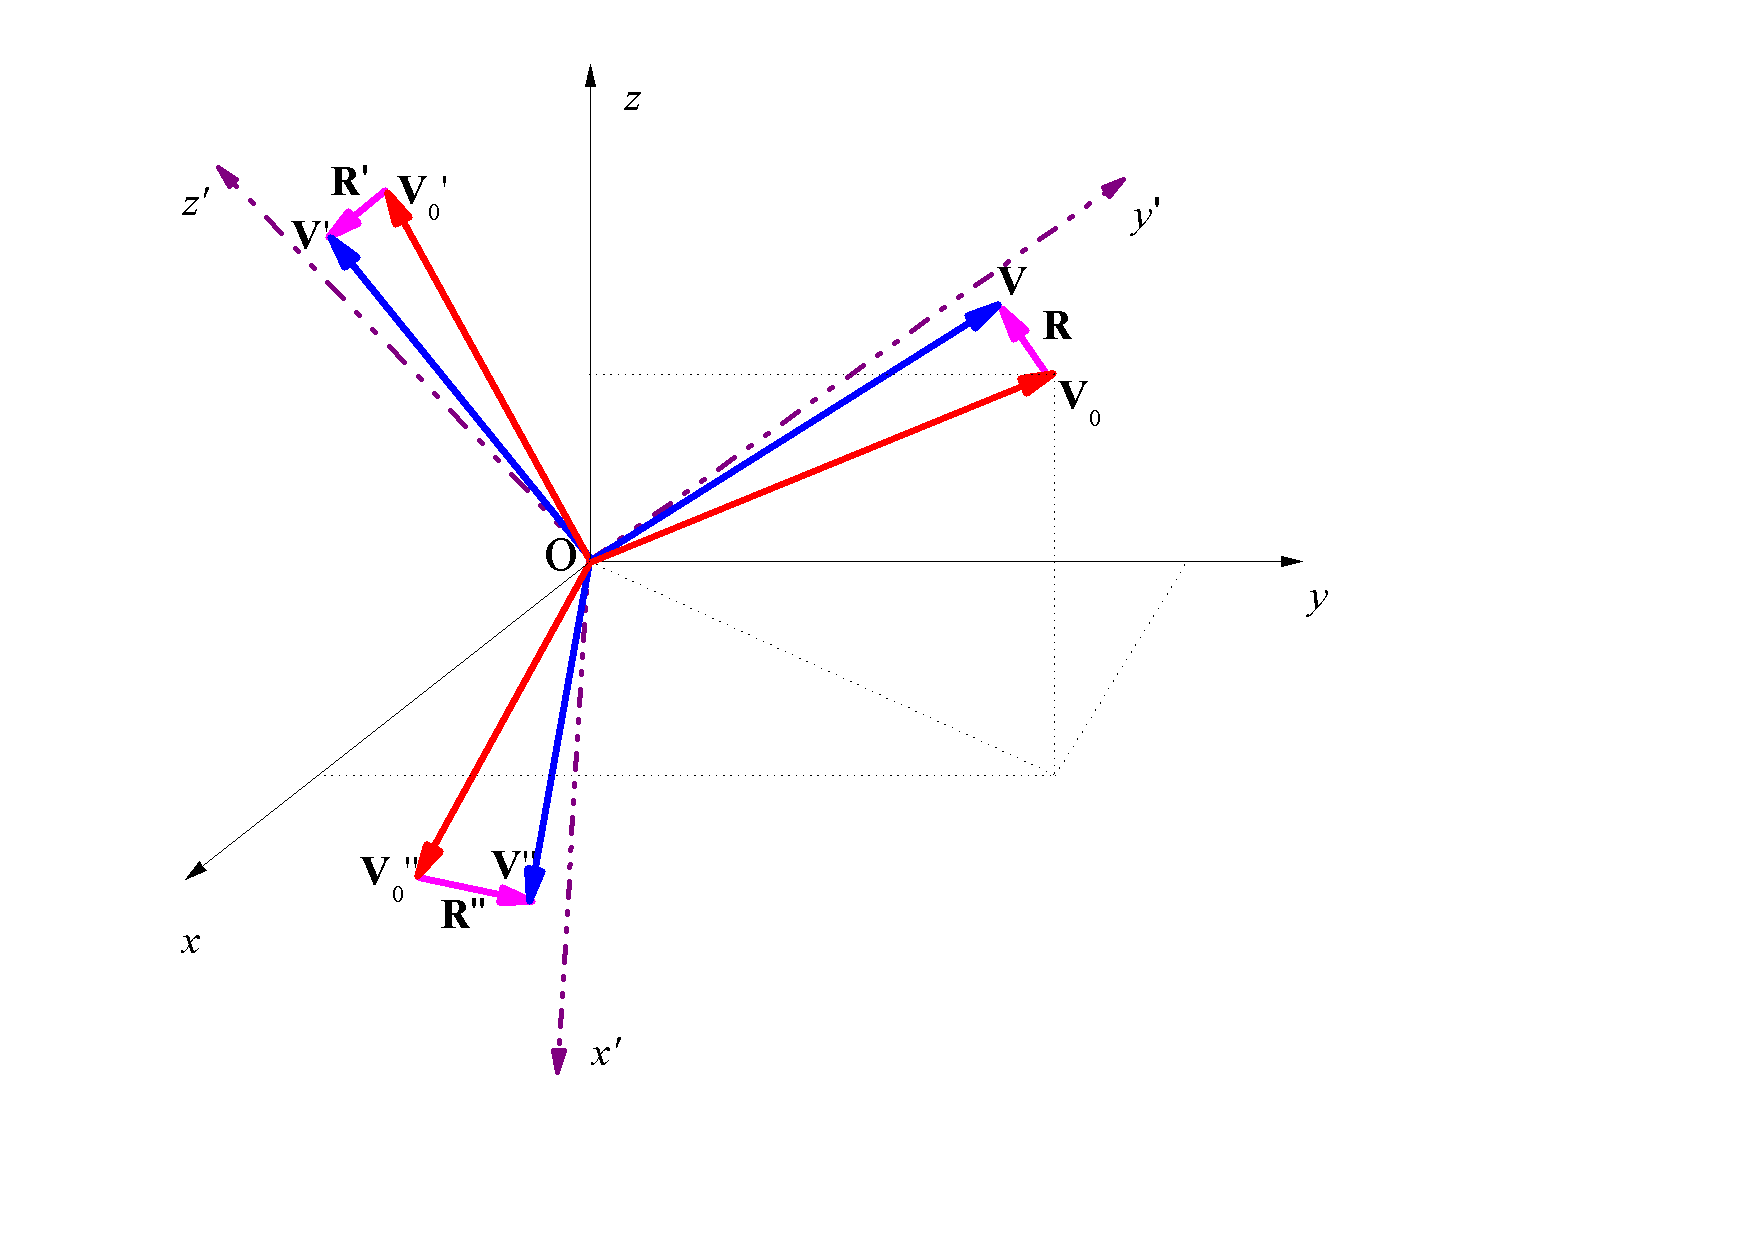
\includegraphics[height=2.5in,width=3.5in,viewport=0 0 850 590,clip]{Figures/Coordinate_transformation.png}
\label{decent_CG}
\caption{\tiny \textrm{Schematic illustration of searching for the eigenvalue of a vector.}}%(与文献\cite{EPJB33-47_2003}图1对比)
\end{figure}
}

\frame
{
	\frametitle{\textrm{Krylov}子空间与矩阵迭代}
	对于矩阵$\mathbf{A}$,取任意矢量$\psi_0$(要求归一),构造矢量$\psi_1$(同样要求归一,并与$\psi_0$正交),满足
	\begin{displaymath}
		\mathbf{A}\psi_0=a_0\psi_0+b_0\psi_1
	\end{displaymath}
	由此确定$a_0$、$b_0$、$\psi_1$
	\begin{displaymath}
		\begin{aligned}
			a_0&=\langle\psi_0|\mathbf{A}|\psi_0\rangle\\
			b_0\psi_1&=\mathbf{A}\psi_0-a_0\psi_0\\
			||\psi_1||&=1
		\end{aligned}
	\end{displaymath}
	进而可构造$\psi_2$:
	\begin{displaymath}
		\mathbf{A}\psi_1=c_1\psi_0+a_1\psi_1+b_1\psi_2
	\end{displaymath}
	要求$\psi_2$与$\psi_0$、$\psi_1$正交归一条件,确定$\psi_2$,$a_1$,$b_1$,$c_1$
}

\frame
{
	\frametitle{\textrm{Krylov}子空间与矩阵迭代}
	根据递推关系有
	\begin{displaymath}
		\mathbf{A}\psi_p=\sum_{q=0}^{p-1}c_p^{(q)}\psi_q+a_p\psi_p+b_p\psi_{p+1}
	\end{displaymath}
	这里$\psi_{p+1}$将与所有之前的$\psi_q$(\textrm{processors})正交

	利用矩阵$\mathrm{A}$的\textrm{Hermitian},因此对于$q<p-1$各项,可有等式
	\begin{displaymath}
		c_p^{(q)}=\langle\psi_q|\mathbf{A}\psi_p\rangle=\langle\mathbf{A}\psi_q|\psi_p\rangle=0
	\end{displaymath}
	即矢量$\psi_p$垂直于矢量$\mathbf{A}\psi_q$,由此可得
	\begin{displaymath}
		c_p^{(p-1)}=\langle\psi_{p-1}|\mathbf{A}\psi_p\rangle=\langle\mathbf{A}\psi_{p-1}|\psi_p\rangle=b_{p-1}
	\end{displaymath}
	经过$p$步迭代后
	\begin{displaymath}
		\mathbf{A}\psi_p=b_{p-1}\psi_{p-1}+a_p\psi_p+b_p\psi_{p+1}
	\end{displaymath}
	这里$\psi_{p+1}$要求与$\psi_p$和$\psi_{p-1}$满足正交归一条件
}

\frame
{
	\frametitle{矩阵对角化的\textrm{Lanczos~}算法}
	因此\textcolor{blue}{矩阵$\mathbf{A}$可以用$\psi_p$(称为\textrm{Lanczos}矢量)为基组表示成三对角阵形式}(稀疏矩阵)
	\begin{displaymath}
		\mathbf{A}^p=\begin{pmatrix}
			a_1 & b_2 & & & & \\
			b_2 & a_2 &b_3 & &\raisebox{0.8ex}[0pt]{\huge{0}} &\\
&b_3 &a_3 &\ddots & & \\
& &\ddots &\ddots &b_{p-1} & \\
& & &b_{p-1} &a_{p-1} &b_{p}\\
&\raisebox{0.8ex}[0pt]{\huge{0}} & & &b_{p} &a_{p}
		\end{pmatrix}
	\end{displaymath}
	不难看出,\textcolor{blue}{经过$p$次\textrm{Lanczos}迭代,当$b\rightarrow0$即达到收敛,意味着此时$p\times p$三对角阵$\mathbf{A}^p$的本征值也将收敛到矩阵$\mathbf{A}$的本征值}
	\begin{itemize}
		\item 稀疏矩阵$\mathbf{A}^p$可通过快速\textrm{QR}分解得到本征值
		\item 三对角阵的最低和最高本征值随着迭代次数增加收敛最迅速
		\item \textrm{Lanczos}方法适用于少量本征值与剩余本征有较大差值的体系
	\end{itemize}
}

\frame
{
	\frametitle{矩阵对角化的\textrm{Lanczos~}算法}
	大型稀疏矩阵对角化基本思路便是从一个试探向量$\mathbf{c}_0$出发,通过矩阵-向量乘操作\footnote{\fontsize{5.2pt}{1.2pt}\selectfont{由于矩阵是稀疏的,从而可以快速进行矩阵-向量乘这一基本操作(时间复杂度$\mathrm{O}(N^2)$)}},同时保持矩阵的稀疏性,使得试探向量逐渐收敛到目标特征向量(往往是基态对应的特征向量)

	{\fontsize{6.2pt}{1.2pt}\selectfont{
		本征值求解对应如下优化问题
		\begin{displaymath}
			\lambda_{\min}=\mathrm{min}_{\mathbf{c}}\rho(\mathbf{c})=\mathrm{min}_{\mathbf{c}}\dfrac{\mathbf{c}^\mathbf{H}\mathbf{c}}{\mathbf{c}^T\mathbf{c}}
		\end{displaymath}
		利用最陡下降法求解上述优化问题,则需要计算函数的梯度
		\begin{displaymath}
			\nabla\rho(\mathbf{c})|_{\mathbf{c}=\mathbf{c}_0}=\dfrac2{\mathbf{c}^T\mathbf{c}}(\mathbf{H}\mathbf{c}_0-\rho(\mathbf{c}_0)\mathbf{c}_0)
		\end{displaymath}
		实际计算中无需求出梯度并作精确搜索,因为\textcolor{blue}{解一定在\textrm{Krylov}子空间$\mathrm{span}(\mathbf{c}_0,\mathbf{H}\mathbf{c}_0)$内;~只需计算这两个向量之间的哈密顿矩阵元,并对角化所得到的小矩阵便相当于做了一步最速下降法}

		经过$k$步迭代之后所得到的解在子空间$\mathrm{span}(\mathbf{c}_0,\mathbf{H}\mathbf{c}_0,\cdots),\mathbf{H}^k\mathbf{c_0}$

		因此\textcolor{magenta}{大型矩阵对角化的问题,转化为子空间内矩阵对角化的问题}

		选取合适的初猜,经过若干次迭代之后,子空间内最小特征值可能于真实的最小特征值非常接近\footnote{\fontsize{5.2pt}{1.2pt}\selectfont{子空间内若干个最小特征值都可能于相应的真值非常接近}}

		一般地,$k$次迭代后第$j$个特征向量写成
		\begin{displaymath}
			\mathbf{c}_j^{(k)}=\sum_{i=0}^kc_{i,j}^{(k)}\mathbf{H}^i\mathbf{c}_0
		\end{displaymath}
	}}
}

\frame
{
	\frametitle{矩阵迭代对角化}
	稀疏矩阵求解的\textrm{Lanczos}优化过程,只变动一个分量$\mathbf{c}_I$的前提下
	\begin{displaymath}
		\dfrac{\partial\rho}{\partial\mathbf{c}_I}\bigg|_{\mathbf{c}_I+\delta_I}=0
	\end{displaymath}
	是可以精确求解的,其解为
	\begin{displaymath}
		\delta_I=(\rho(\mathbf{c}_0)-\mathbf{H}_{II})^{-1}\mathbf{q}_I\qquad\mbox{这里}\mathbf{q}=(\mathbf{H}-\rho\mathbf{I})\mathbf{c}_0
	\end{displaymath}
	不难看出,矢量$\mathbf{q}$就对应\textrm{Jacobi}迭代中用于判断收敛的残差矢量

更一般地,求解方程
	\begin{displaymath}
		\dfrac{\partial\rho}{\partial\mathbf{c}}\bigg|_{\mathbf{c}+\mathbf{\delta}}=0
	\end{displaymath}
	将方程展开到二阶近似,不难有
	\begin{displaymath}
		(\rho-\mathbf{H}_{II})\delta_I\approx \mathbf{q}_I+\sum_{J\neq I}\delta_J+(\rho-\lambda)\mathbf{c}_I
	\end{displaymath}
	实际计算中选则$\delta_I=(\rho(\mathbf{c}_0)-\mathbf{H}_{II})^{-1}\mathbf{q}_I$并不是方程的解的好的近似,\textcolor{purple}{好处是计算比较简单}
}

\frame
{
	\frametitle{\textrm{Block-Davison algorithm}}
	\textrm{Davidson}方法是求解大型稀疏矩阵的少量本征值问题提出来的,结合了\textrm{Lanczos}优化和\textrm{Jacobi}迭代的优点,简言之就是改进初猜,不用$\mathbf{H}\mathbf{c}_0$,而改用计算简单的$\delta_I=(\rho(\mathbf{c}_0)-\mathbf{H}_{II})^{-1}\mathbf{q}_I$形式
	\vskip 10pt
	应用\textrm{Davison}方法可以快速地依次求解稀疏矩阵的少量本征值和本征矢,将该方法推广为同时求解若干个本征态,即块-\textrm{Davidson}方法
	{\fontsize{6.2pt}{1.2pt}\selectfont{
		\begin{itemize}
			\item 选取合适数目正交归一的向量$\mathbf{c}_1,\mathbf{c}_2,\cdots, \mathbf{c}_n$作为初猜子空间的基组, 计算并储存向量$\mathbf{H}\mathbf{c}_i$和矩阵元$\mathbf{H}=\langle\mathbf{c}_i|\mathbf{H}|\mathbf{c}_j\rangle$ 
			\item 对角化矩阵,得到本征值$\lambda^{n}$和本征矢$\mathbf{a}^{n}$
			\item 构造残量矢量$\mathbf{q}_M=(\mathbf{H}-\lambda^{(M)}\mathbf{I})\mathbf{a}^{(M)}~\mbox{其中}\mathbf{a}^{(M)}=\sum\limits_{i=1}^M a_i^{(M)}\mathbf{a}_i$
			\item 根据模长$||\mathbf{q}_M||$判断迭代收敛情况
			\item 构造$\delta_{I,M+1}=(\lambda^{(M)}-\mathbf{H}_{II})^{-1}\mathbf{q}_{I,M}$,与此前的基组正交归一化,得到$\mathbf{c}_{M+1}$
			\item 计算矩阵元$\mathbf{H}_{i,M+1}\quad i=1,2,\cdots, M+1$
			\item 对角化矩阵得到新的本征值和本征矢量,继续迭代
		\end{itemize}
	}}
}

\frame
{
	\frametitle{\textrm{RMM-DIIS}}
	{\fontsize{7.2pt}{1.2pt}\selectfont{前述矩阵迭代对角化方法的优化策略都是
	\begin{itemize}
		\item 通过迭代优化得到最小本征值(极值)
		\item 利用本征态正交,依次获得其他各本征态和本征值
	\end{itemize}}}
	{\fontsize{7.2pt}{1.2pt}\selectfont{\textrm{RMM-DIIS~(Residual Minimization Method by Direct Inversion in the Iterative Subspace)}\footnote{\fontsize{5.2pt}{1.2pt}\selectfont{\textrm{RMM-DIIS}的得名源自该方法的提出者\textrm{Pulay}:~该方法的基本思想是在历次迭代产生的矢量构成的完整\textrm{Krylov}子空间内,完成对残矢的最小化}}方法则可以不用引入正交条件而得到多个本征值,\textcolor{purple}{因为该方法最小化的不是本征值而是残矢}}}\\
	{\fontsize{5.2pt}{1.2pt}\selectfont{
		其基本思想概要:~在$n$维\textrm{Krylov}子空间内,生成矢量
		\begin{displaymath}
			\psi^{n+1}=c_0\psi^0+\sum_{j=1}^{n+1}c_j\delta\psi^{j}
		\end{displaymath}
		通过改变选取一套合适的系数$c_j$来完成$\psi^{n+1}$的残矢$R^{n=1}$的最小化。\textcolor{blue}{等价于$c_j$由$\{\psi^0,\psi^1,\cdots,\psi^n\}$构成的\textrm{Krylov}子空间内求\textrm{Hermitian}本征值问题}
		\begin{displaymath}
			\sum_{j=1}^n\langle R^i|R^j\rangle c_j=\varepsilon\sum_{j=1}^n\psi^i|\mathbf{S}|\psi^j\rangle c_j
		\end{displaymath}
		每迭代一次,子空间引入一个新波函数$\psi$和一个新残矢$R(\psi)$
		\begin{itemize}
			\item \textrm{RMM-DIIS}的计算量瓶颈将是后续的逐个矩阵-向量乘操作$\textrm{H}\psi$
%				\\因此要避免直接用\textrm{RMM-DIIS}直接处理大规模本征态~(但可以是大体系中的少量本征态)
			\item 只要内存许可,\textrm{RMM-DIIS}构造的完整的子空间内,构成子空间的矢量本征值都可以求解出来
			\item 因为\textrm{RMM}方法对初猜的矢量敏感(矢量收敛的位置到离初猜较近)
		\end{itemize}
%		\textrm{RMM-DIIS}最大的优点是一次可以得到多个本征态和本征值,而且不需要正交化
	}}
}

\frame
{
	\frametitle{\textrm{VASP}的并行效率}
	与同类型软件相比,\textrm{VASP}有着优异的并行能力
\begin{figure}[h!]
	\vspace{-0.15in}
\centering
%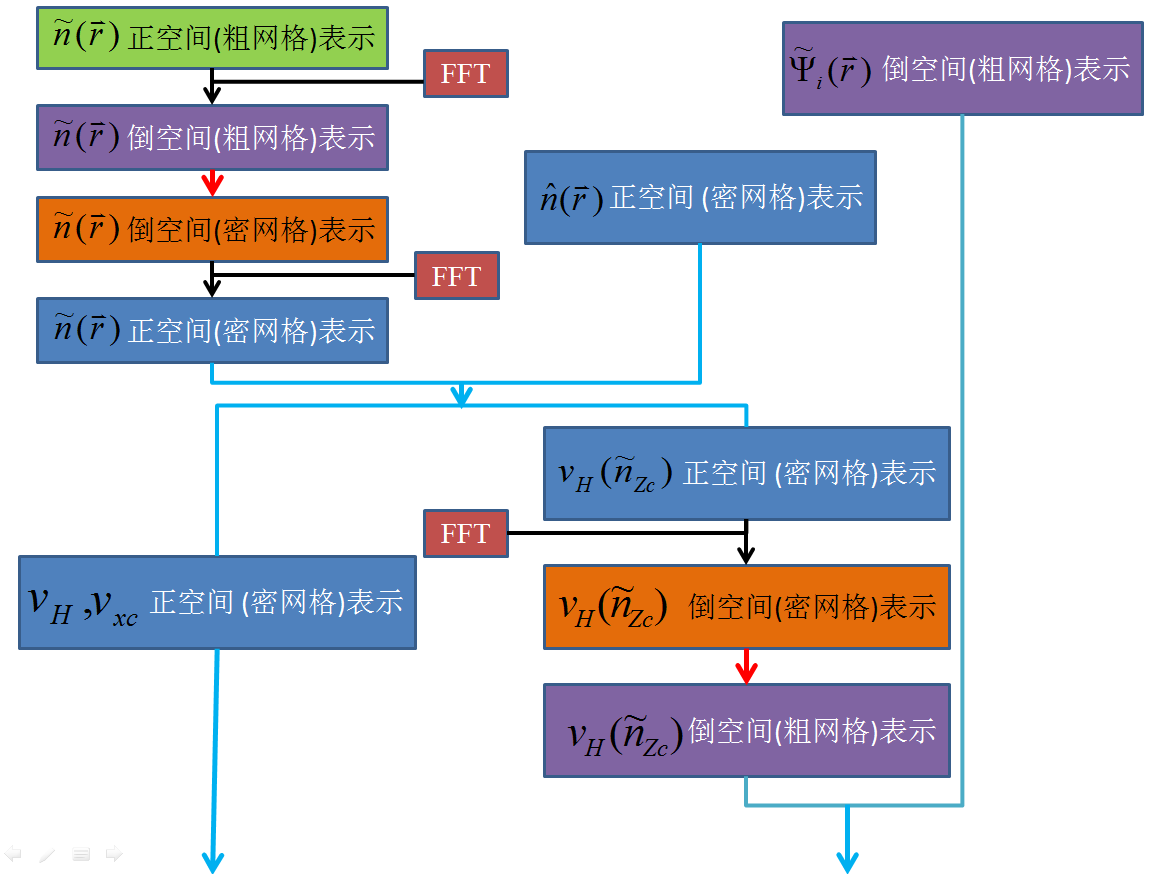
\includegraphics[height=2.7in,width=4.0in,viewport=0 0 1180 875,clip]{Figures/dual_grid.png}
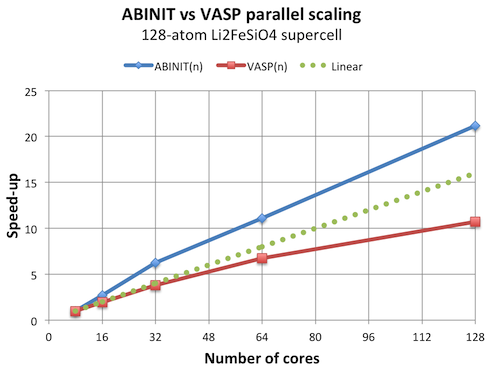
\includegraphics[height=1.55in,width=1.95in,viewport=0 0 240 200,clip]{Figures/VASP-abinit_Li128-1.png}
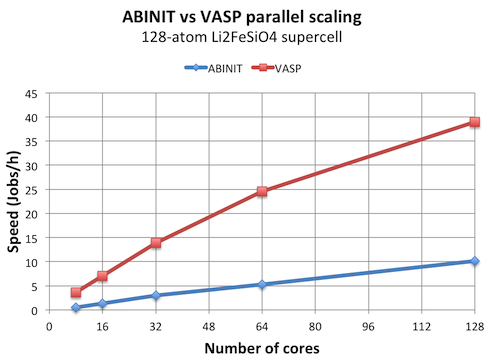
\includegraphics[height=1.55in,width=1.95in,viewport=0 0 240 200,clip]{Figures/VASP-abinit_Li128-2.png}
\caption{\tiny \textrm{The comparison of parallel scaling for ABINIT vs VASP.}}%(与文献\cite{EPJB33-47_2003}图1对比)
\label{ABINIT_vs_VASP}
\end{figure} 
\begin{itemize}
	\item \textrm{VASP}迭代对角化约束了矩阵的维度,减少了对角化过程中的迭代次数,保证了\textrm{MPI}并行的规模和扩展性
	\item \textrm{VASP}实施\textrm{FFT}变换时,保证各节点上处理的网格负载均衡
\end{itemize}
}

\frame
{
	\frametitle{\textrm{VASP}计算的\textrm{FFT}并行实现}
	\begin{itemize}
	     \item 中间层设计:~\textrm{FFT}网格、实空间基组与计算节点的匹配\\
		     \textcolor{red}{通过子程序\textrm{mgrid.F}生成中间层,实现并行负载与计算节点分配的匹配,减少\textrm{FFT}变换和实空间并行的节点间通信}
\begin{figure}[h!]
		\vspace{-0.25in}
	\centering
%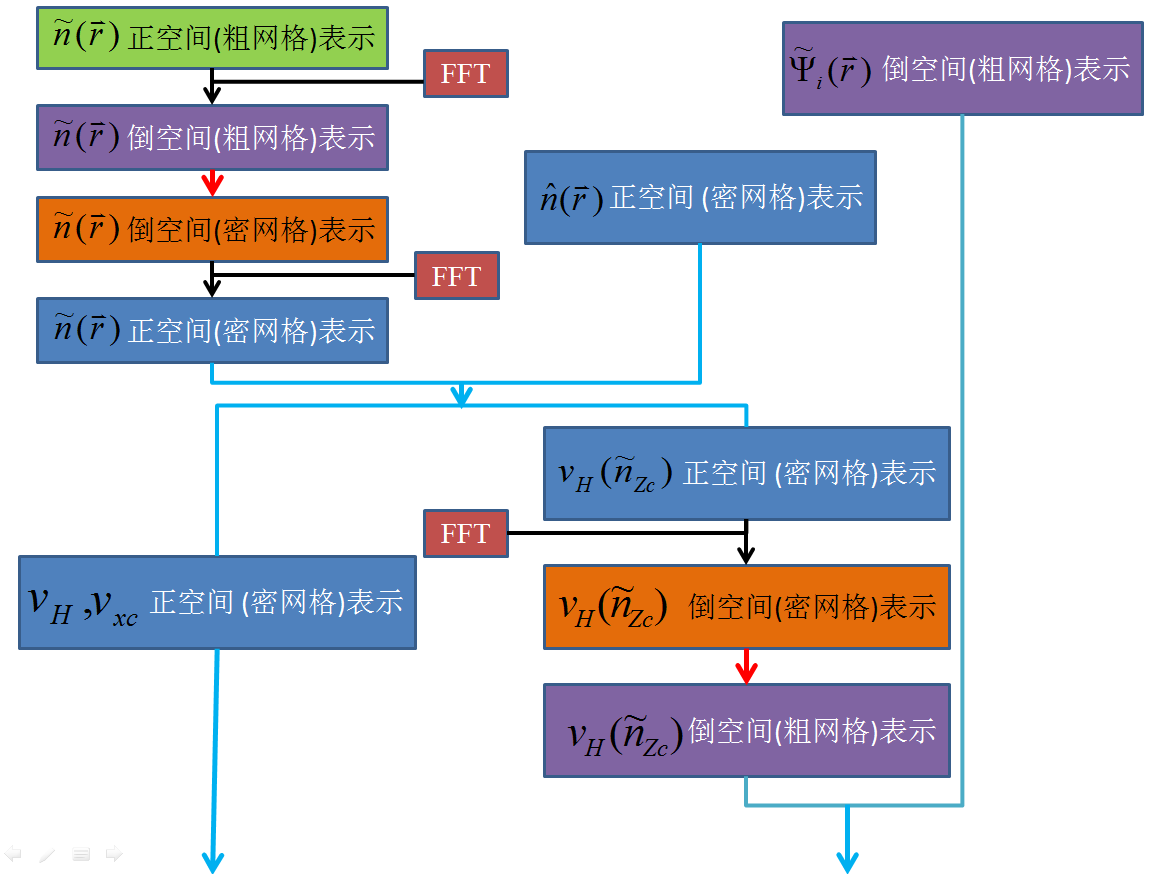
\includegraphics[height=2.7in,width=4.0in,viewport=0 0 1180 875,clip]{Figures/dual_grid.png}
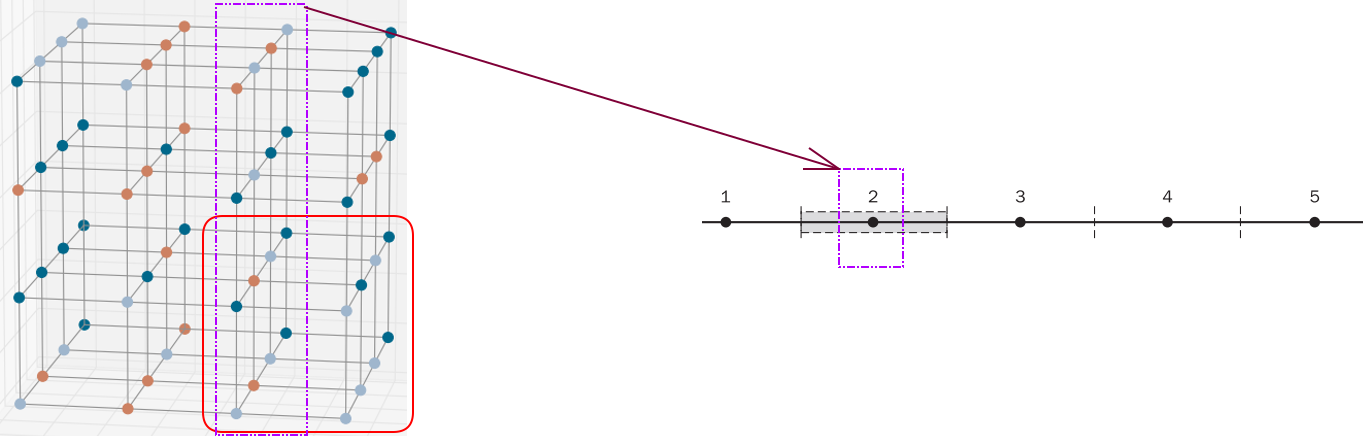
\includegraphics[height=1.0in,width=4.0in,viewport=0 0 1500 450,clip]{Figures/VASP_FFT-MPI_Reciprocal.png}
\vskip 0.5pt
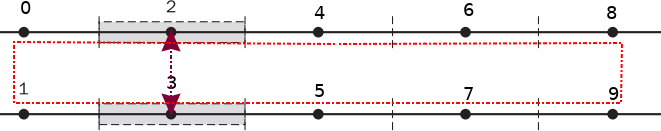
\includegraphics[height=0.7in,width=4.0in,viewport=0 0 730 150,clip]{Figures/VASP_FFT-MPI_Real.png}
\caption{\tiny \textrm{VASP:~ Reciprocal-Real space layout for grids in MPI.}}%(与文献\cite{EPJB33-47_2003}图1对比)
\label{MPI-FFT}
\end{figure} 
	\end{itemize}
}

\frame
{
	\frametitle{\textrm{VASP}的通信开销}
	在高性能的计算队列中,\textrm{VASP}的并行上限可以突破256核,但当并行核数超过百核数量级,并行效率下降非常明显
\begin{figure}[h!]
	\vspace{-0.15in}
\centering
%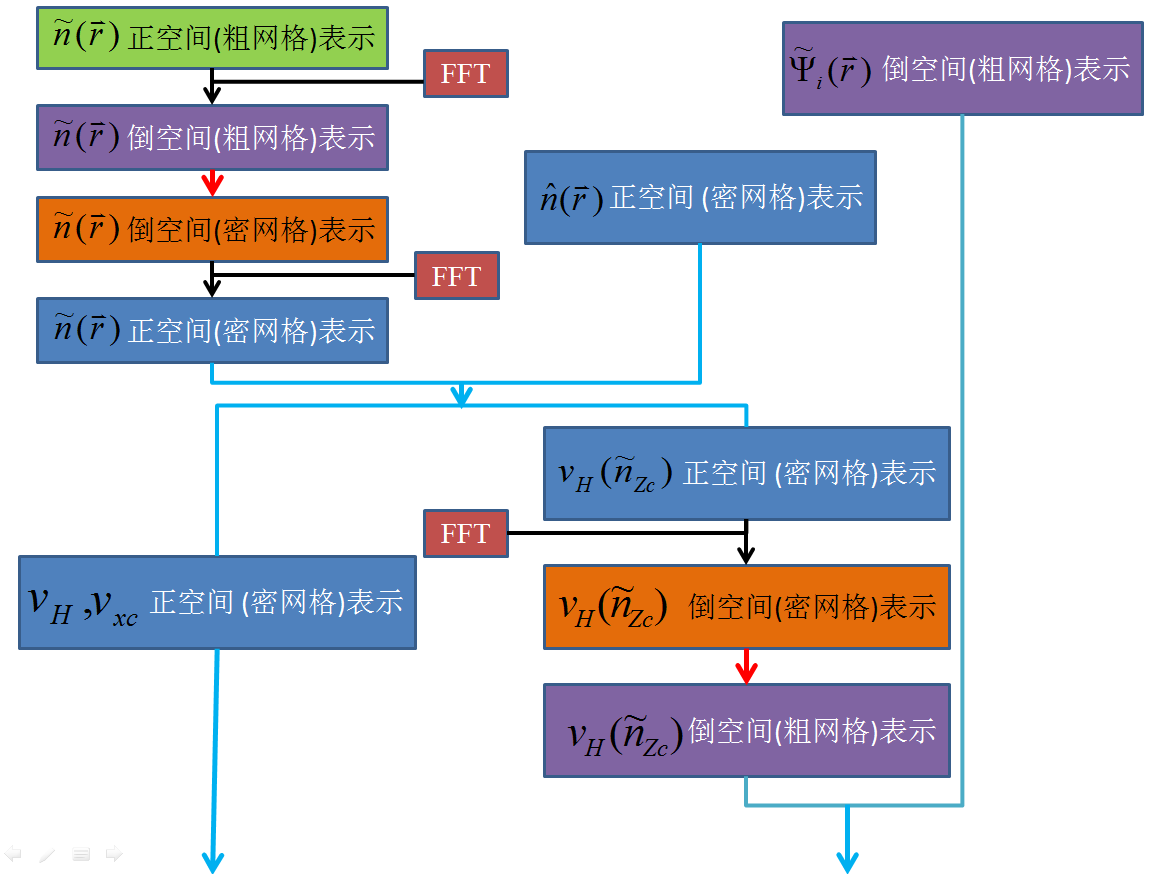
\includegraphics[height=2.7in,width=4.0in,viewport=0 0 1180 875,clip]{Figures/dual_grid.png}
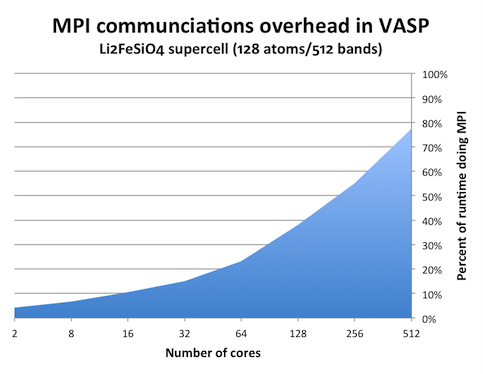
\includegraphics[height=1.55in,width=1.95in,viewport=0 0 240 200,clip]{Figures/VASP-mpi-Li128.png}
\caption{\tiny \textrm{Time spent in MPI calls with increasing the number of ranks in a VASP calculation.}}%(与文献\cite{EPJB33-47_2003}图1对比)
\label{VASP_communication}
\end{figure} 

如能对并行系统与\textrm{VASP}结合作深度改造(如国家超算天津中心方案),\textrm{VASP}的并行扩展可以到$10^4$核级别,但这一改造需要对底层代码和计算框架作较大规模改动
}

\frame
{
	\frametitle{\textrm{VASP}的\textrm{GPU}加速}
\textrm{NVIDIA}多年来致力于\textrm{VASP}的\textrm{GPU}加速,取得了一定的成效
\begin{figure}[h!]
	\vspace{-0.15in}
\centering
%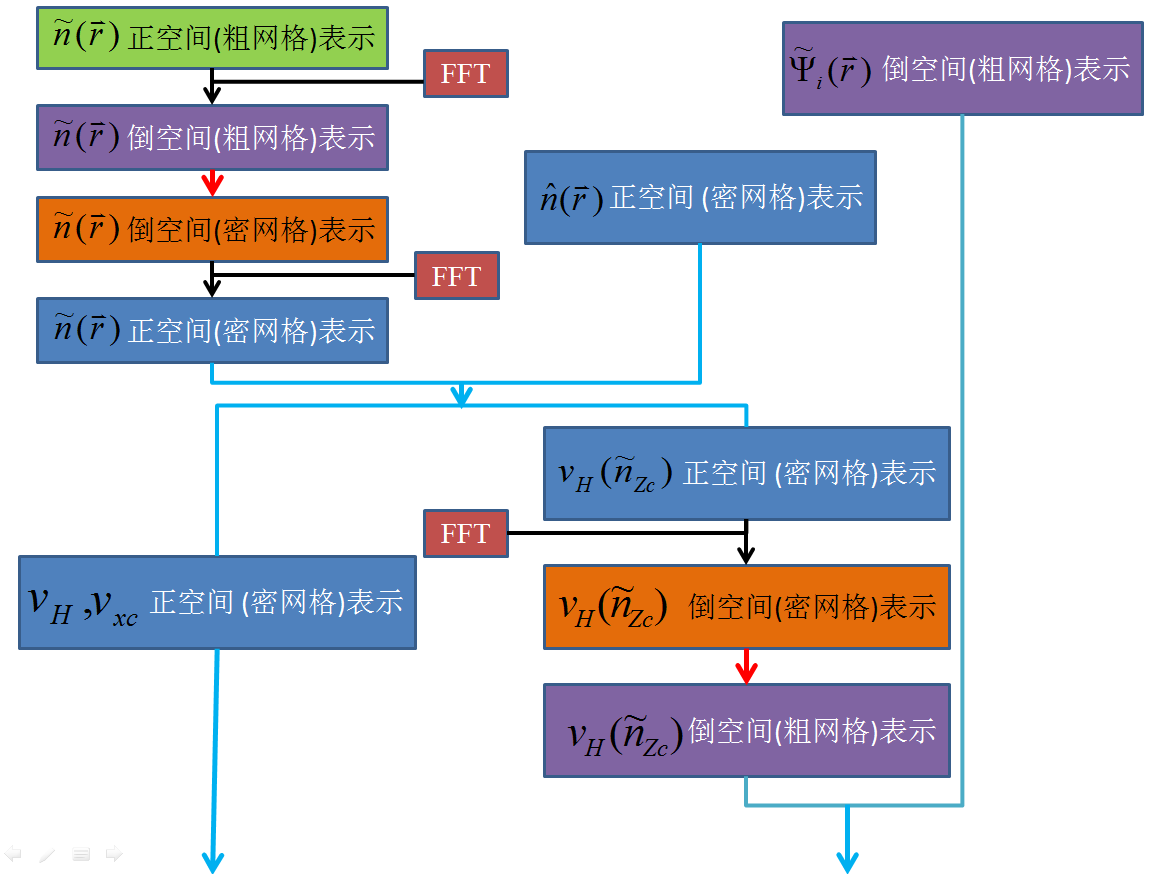
\includegraphics[height=2.7in,width=4.0in,viewport=0 0 1180 875,clip]{Figures/dual_grid.png}
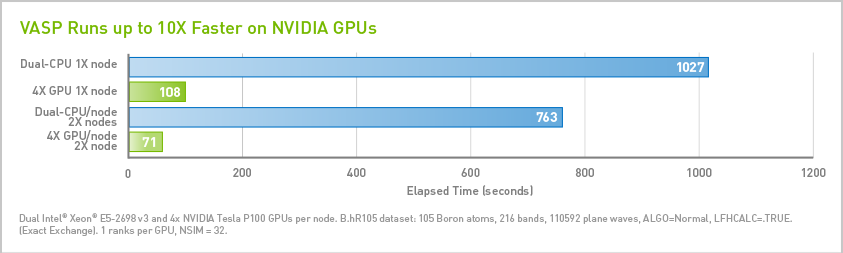
\includegraphics[height=1.2in,width=4.05in,viewport=0 0 850 260,clip]{Figures/VASP-GPU-CPU.png}
\caption{\tiny \textrm{Compare of VASP calculation with GPU and CPU.}}%(与文献\cite{EPJB33-47_2003}图1对比)
\label{VASP_GPU}
\end{figure} 
\begin{itemize}
	\item 通用配置下,\textrm{GPU}对\textrm{VASP}计算有加速效果,一般可提升4$\sim$6倍
	\item 矩阵对角化的并行算法限制了\textrm{GPU}在第一原理计算中的应用
	\item \textrm{GPU}加速的模式主要适合于分子动力学计算
\end{itemize}
}

\subsection{\rm{VASP}软件的主程序结构}
%\frame[allowframebreaks]
\begin{frame}[allowframebreaks]{\textrm{VASP}的主程序结构}
\begin{figure}[h!]
\vskip -10pt
\centering
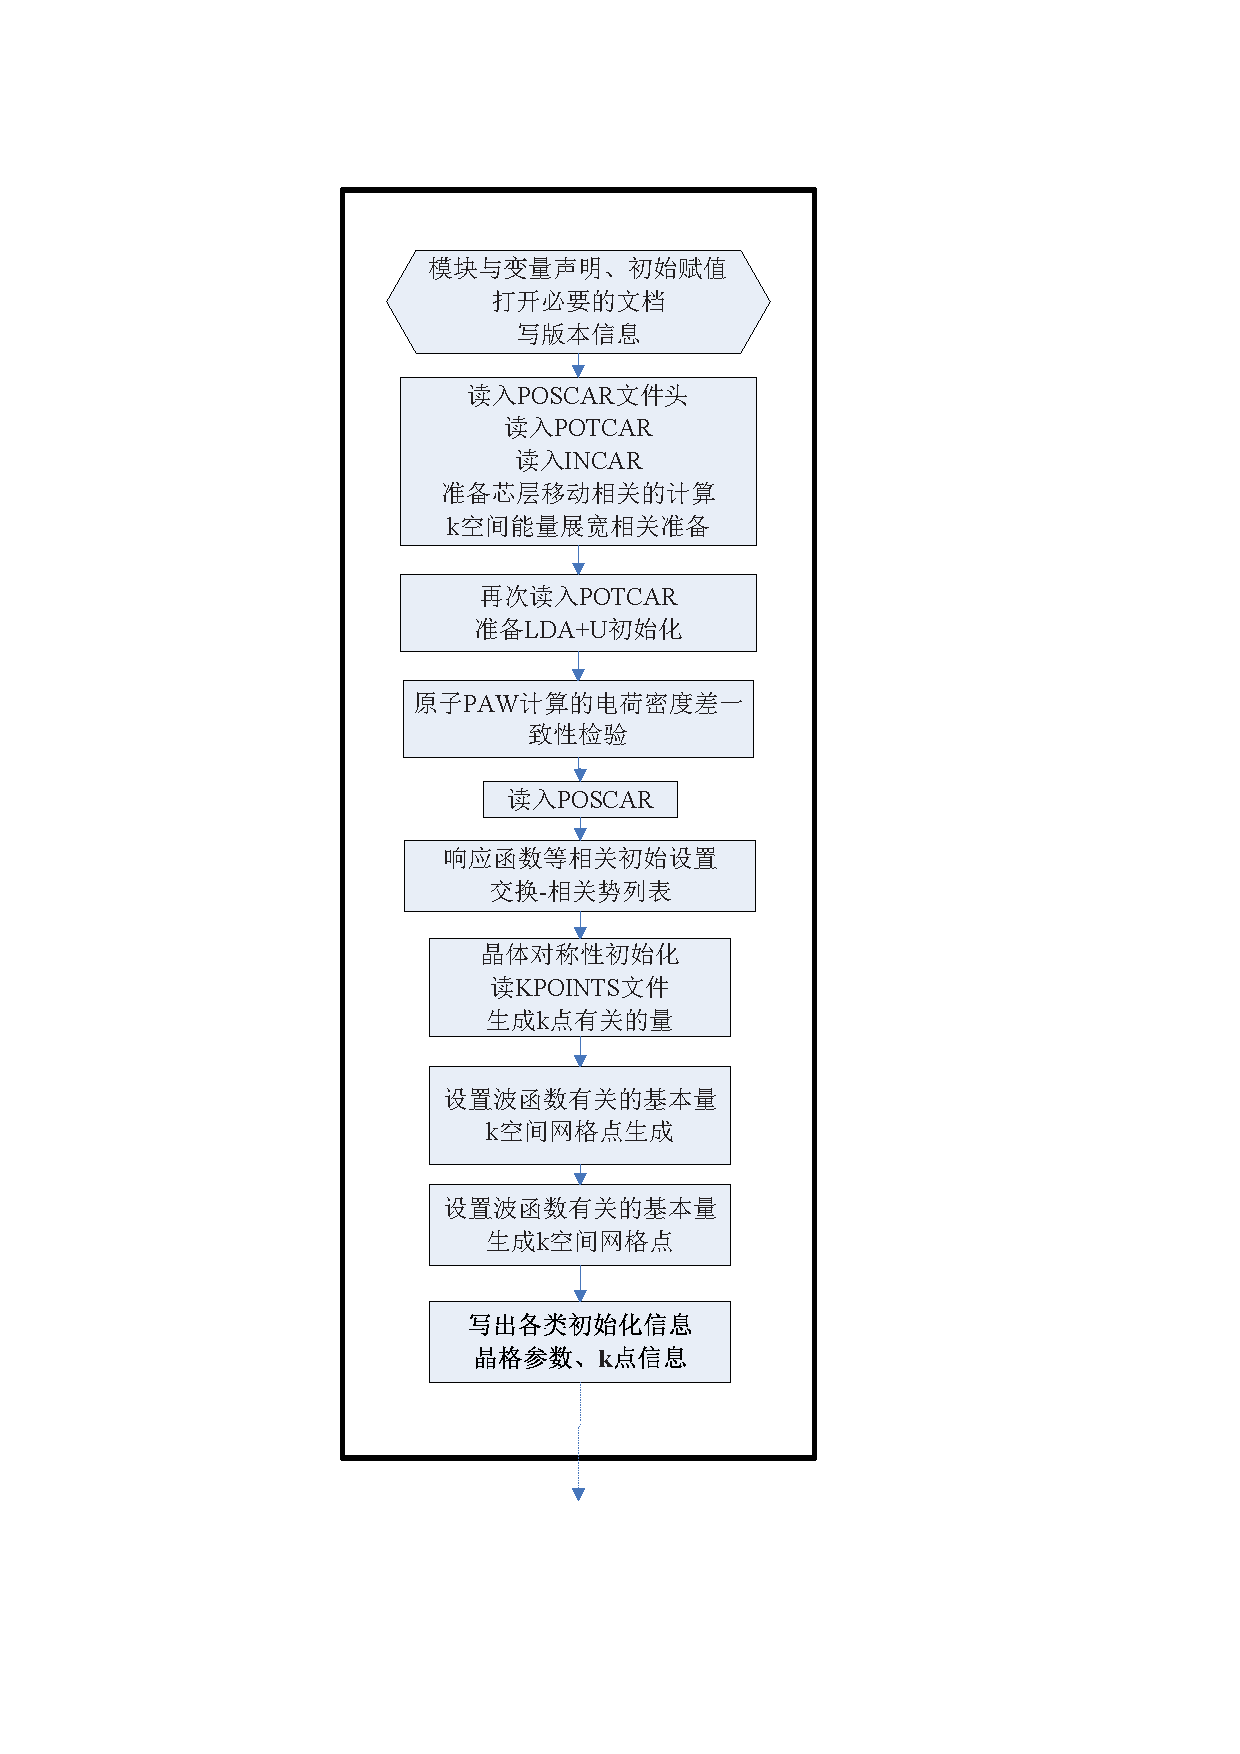
\includegraphics[height=2.65in,width=4.0in,viewport=0 360 562 720,clip]{Figures/VASP_main_Flow-1.png}
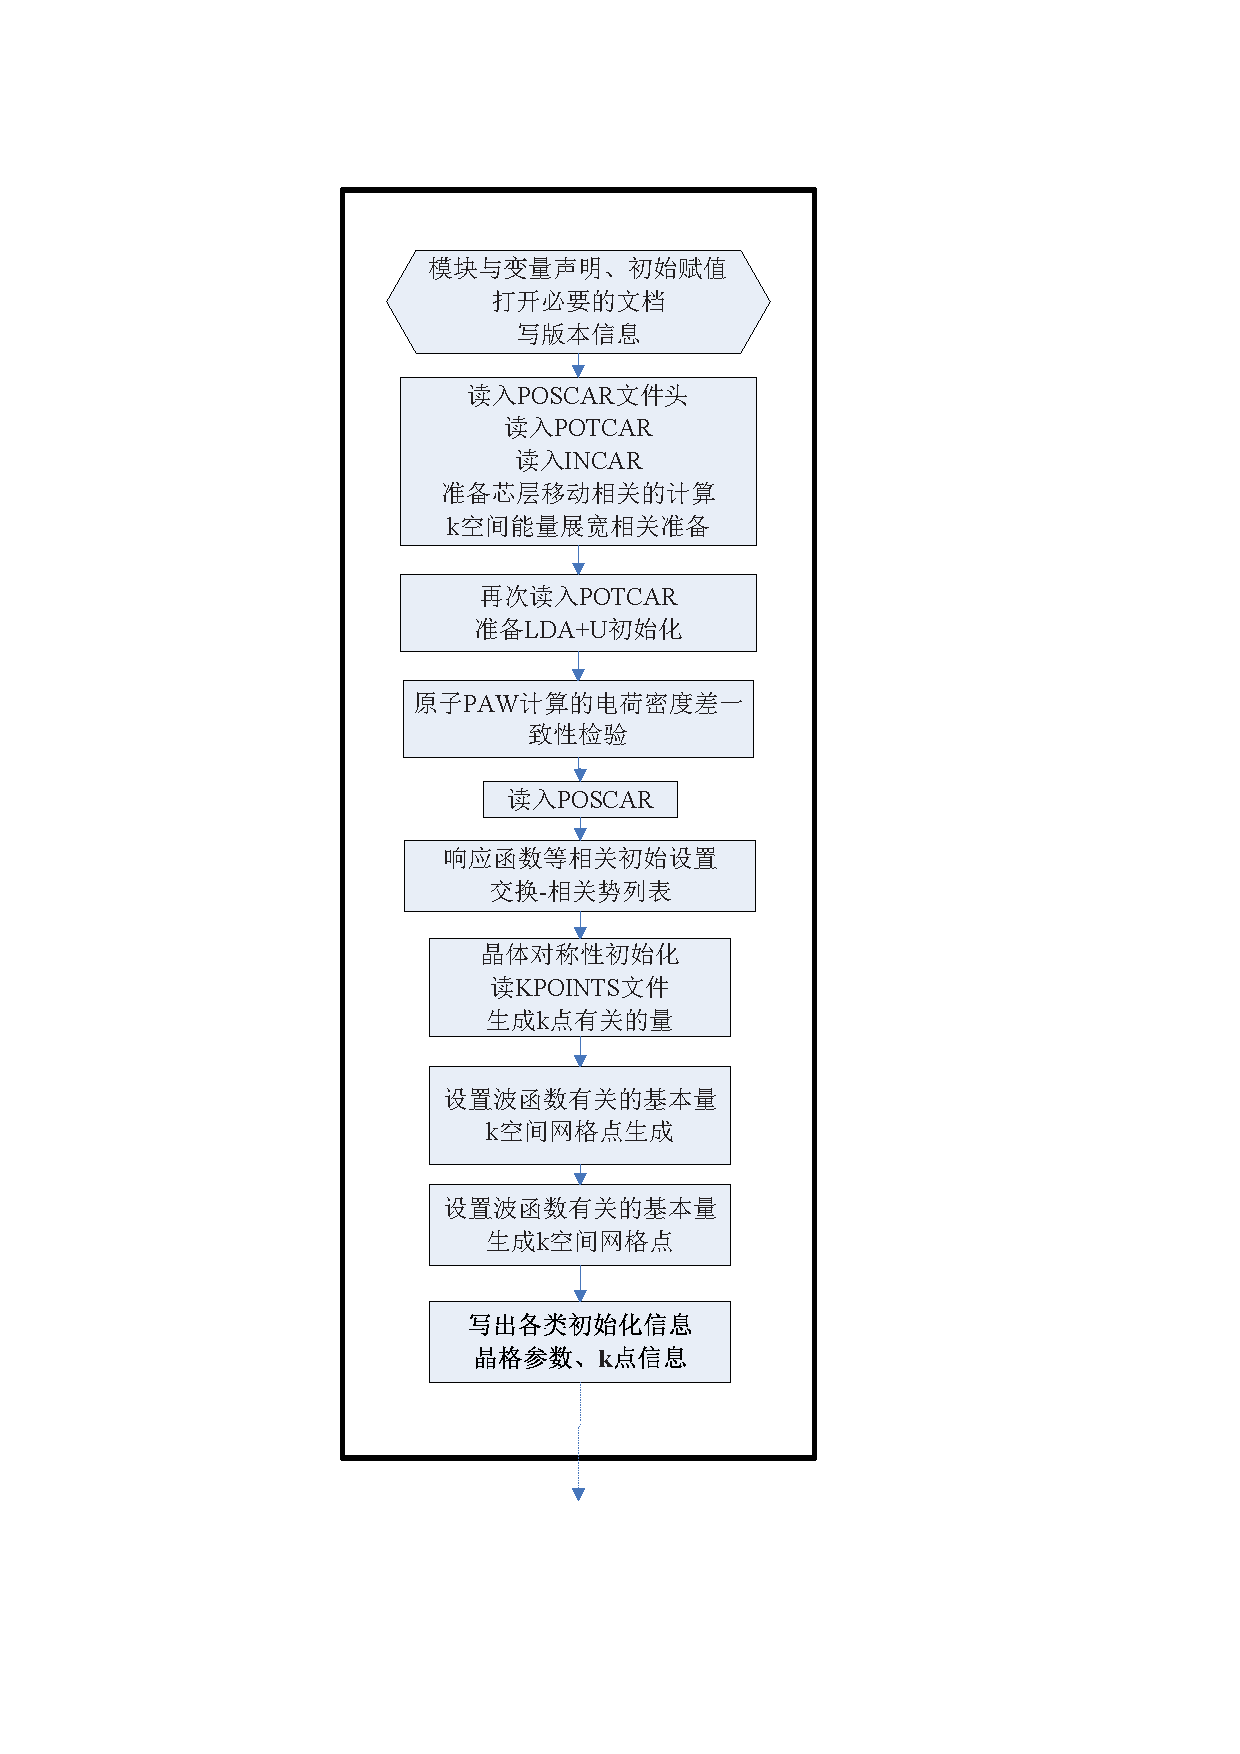
\includegraphics[height=2.65in,width=4.0in,viewport=0 0 562 360,clip]{Figures/VASP_main_Flow-1.png}
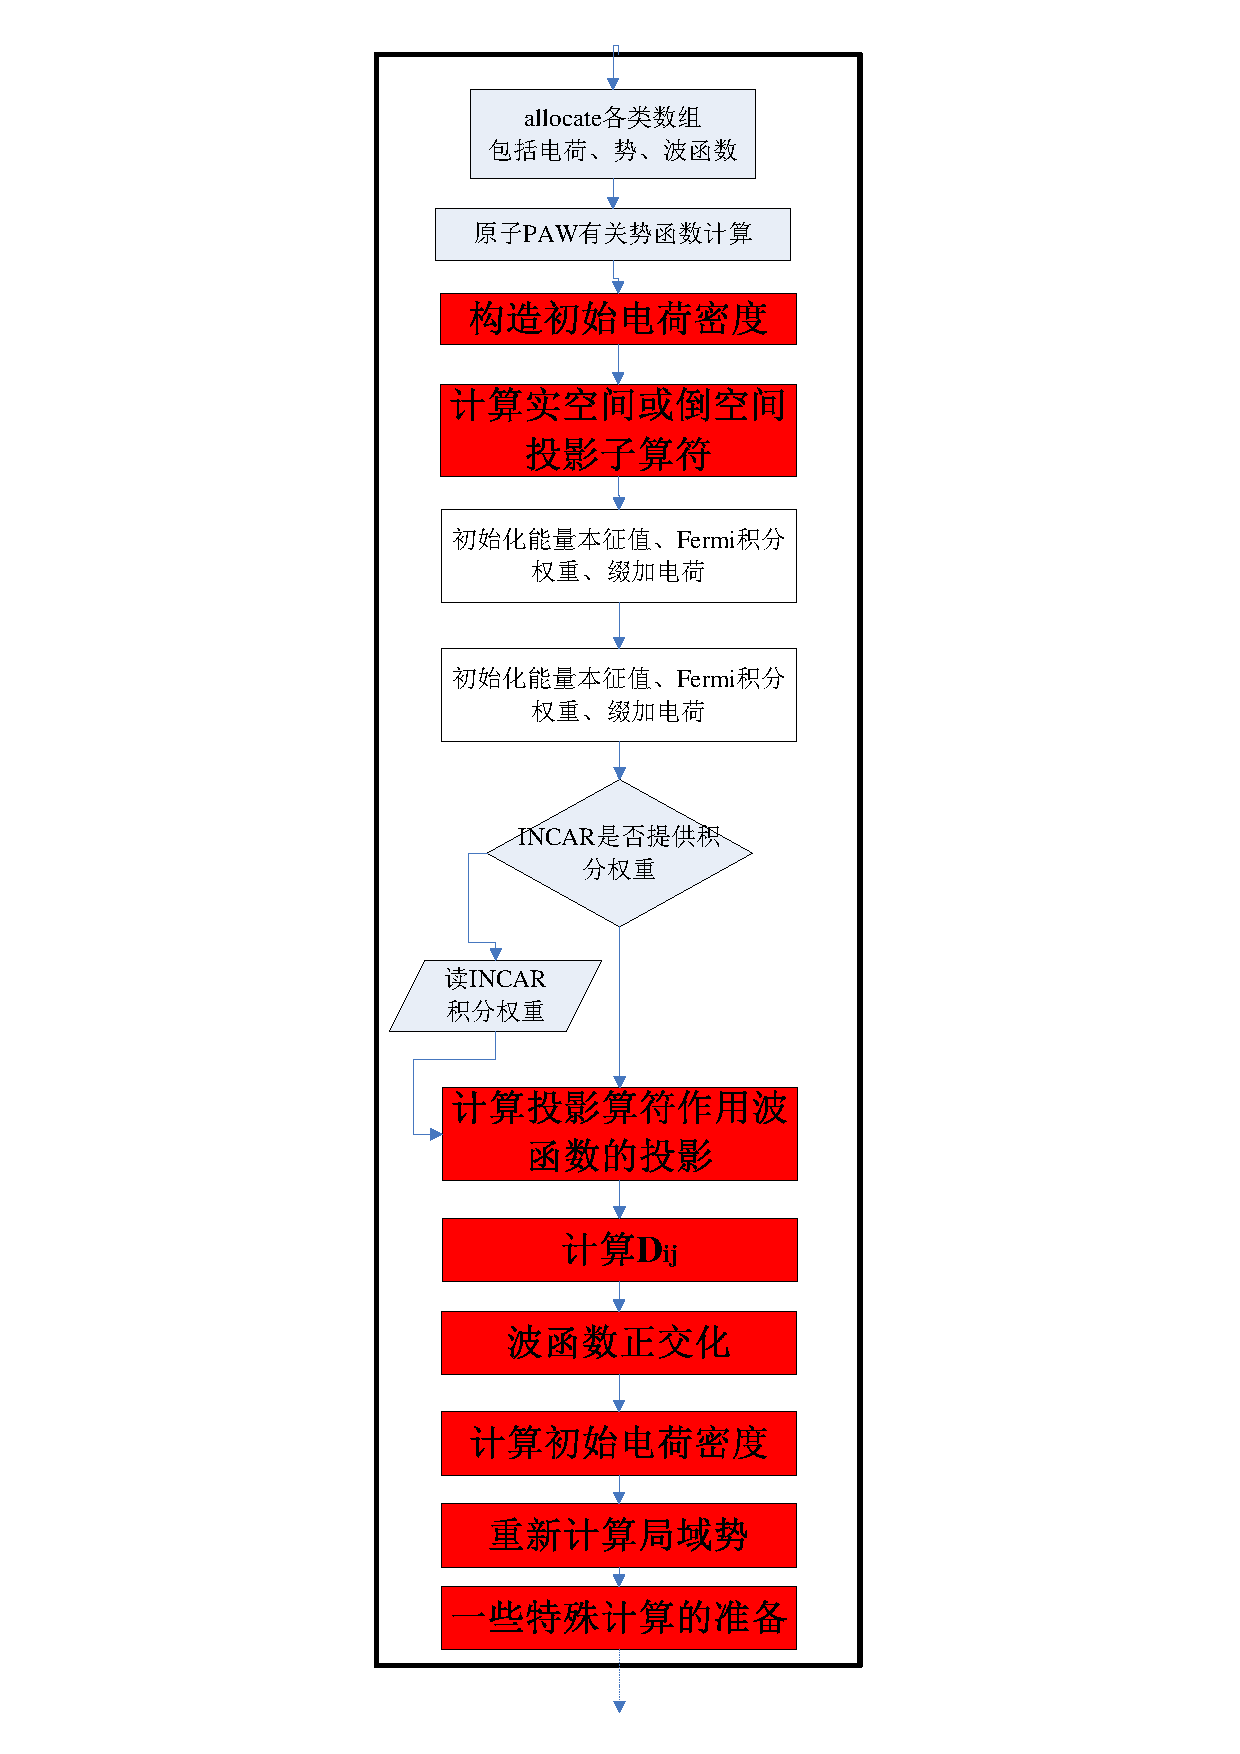
\includegraphics[height=2.35in,width=4.0in,viewport=0 370 562 680,clip]{Figures/VASP_main_Flow-2.png}
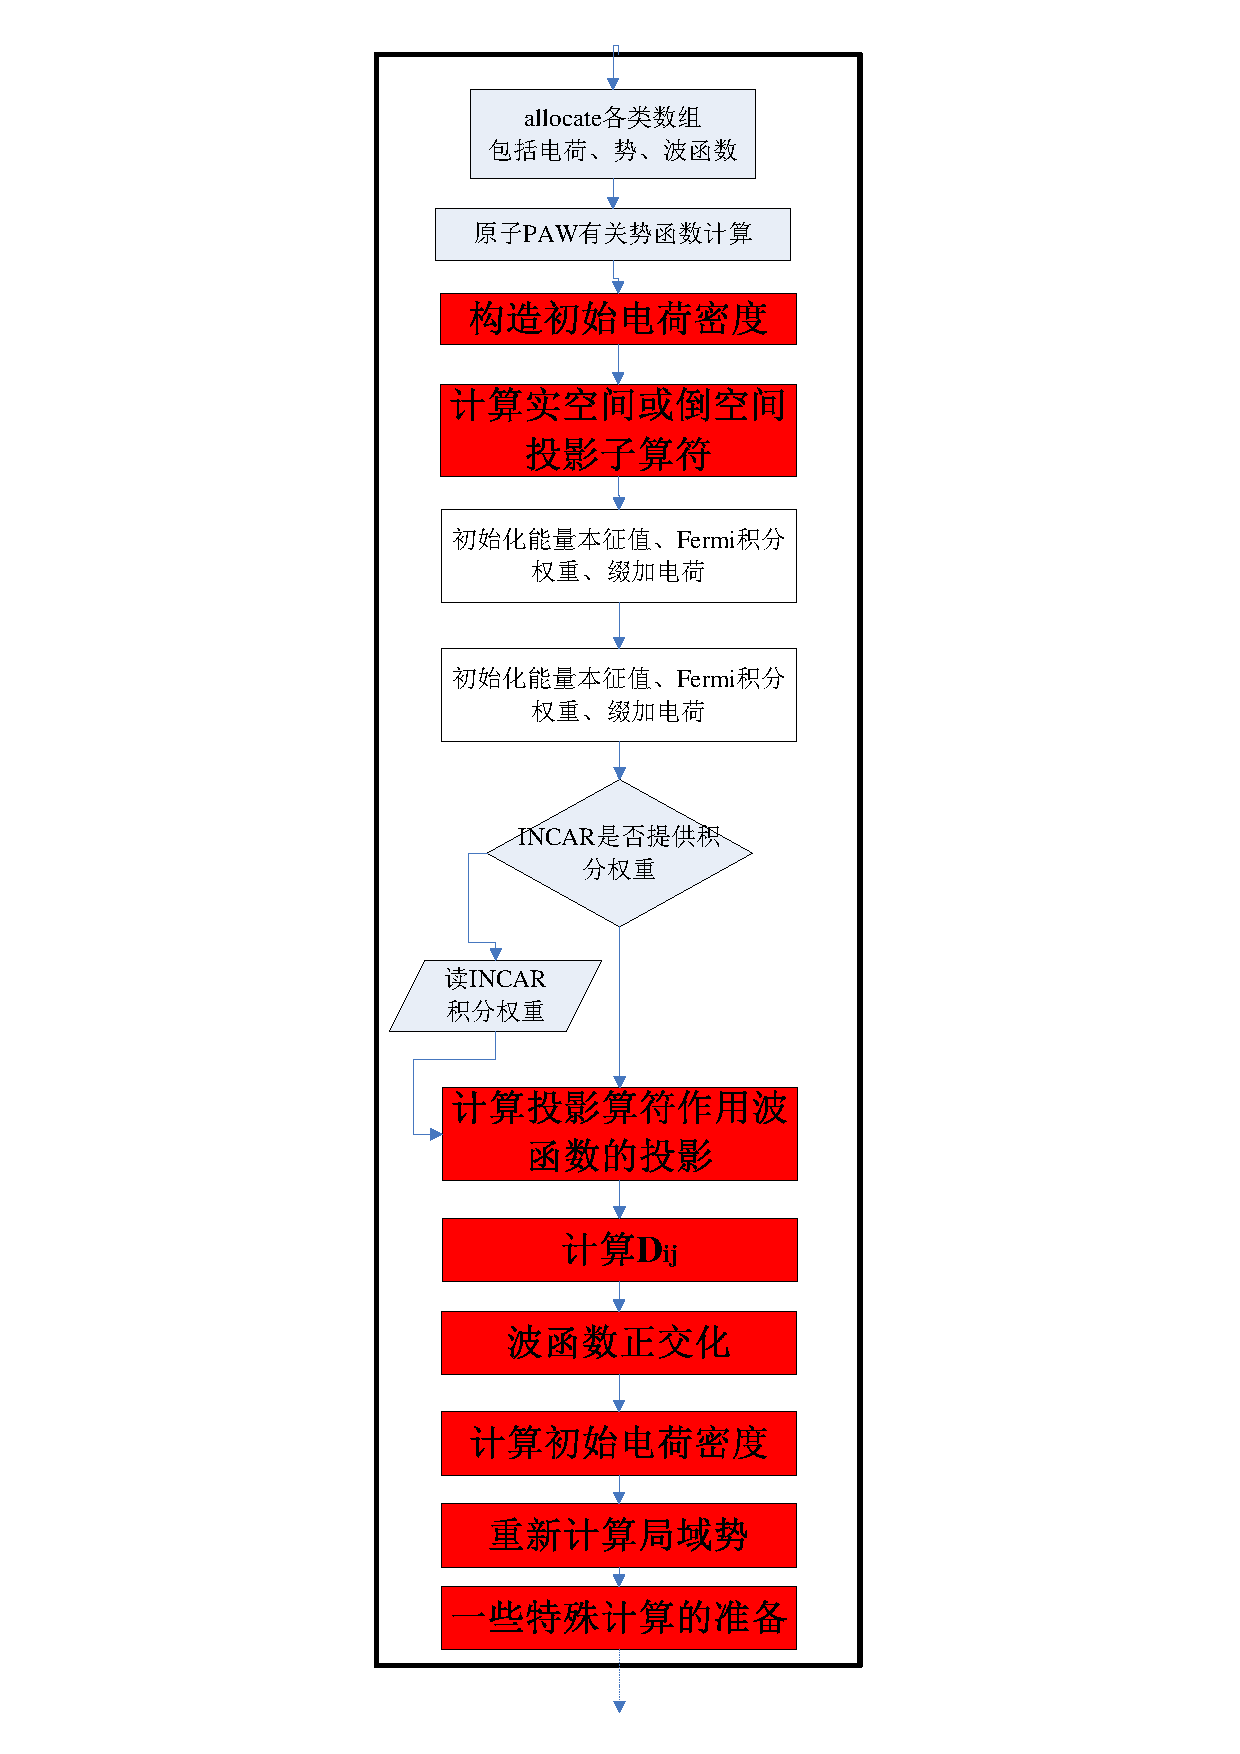
\includegraphics[height=2.50in,width=4.0in,viewport=0 0 562 370,clip]{Figures/VASP_main_Flow-2.png}
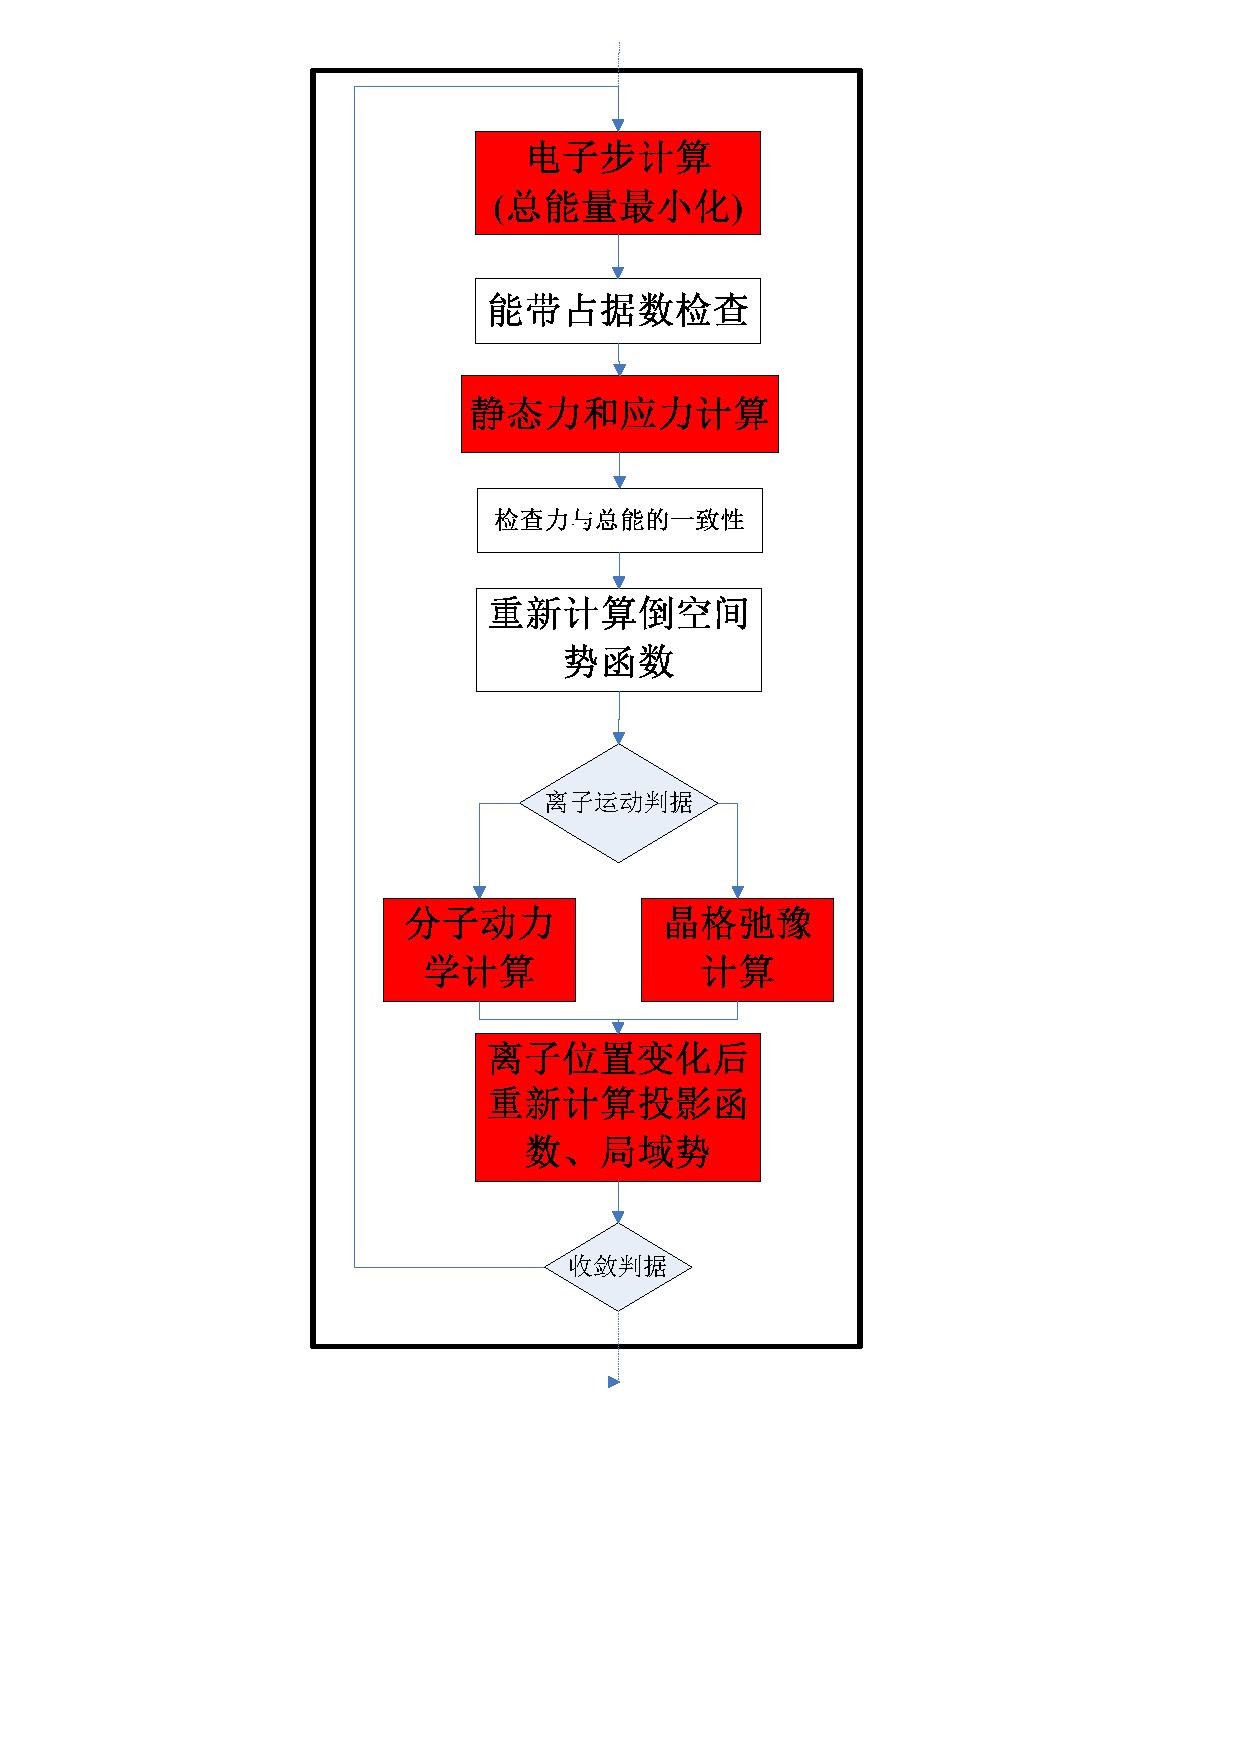
\includegraphics[height=2.45in,width=4.0in,viewport=0 350 562 660,clip]{Figures/VASP_main_Flow-3.png}
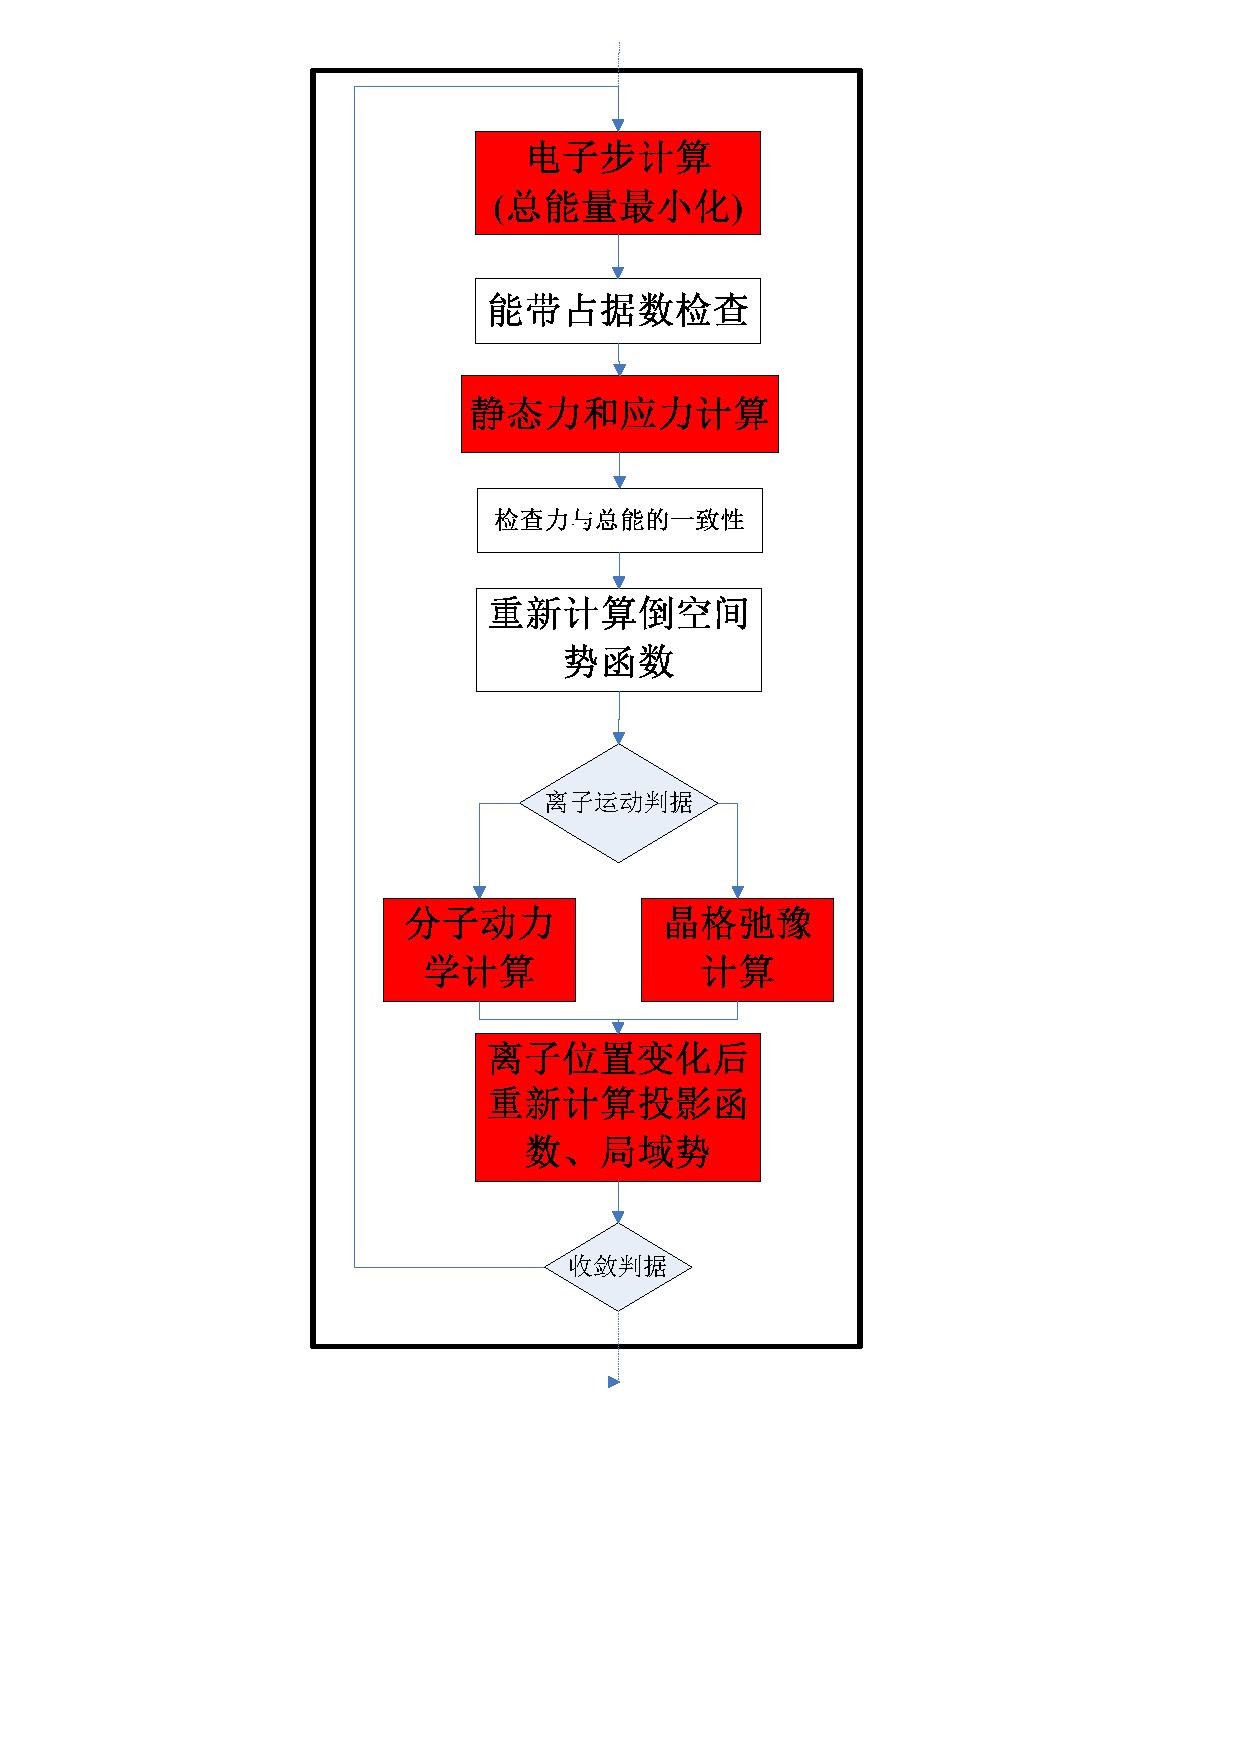
\includegraphics[height=2.50in,width=4.0in,viewport=0 0 562 350,clip]{Figures/VASP_main_Flow-3.png}
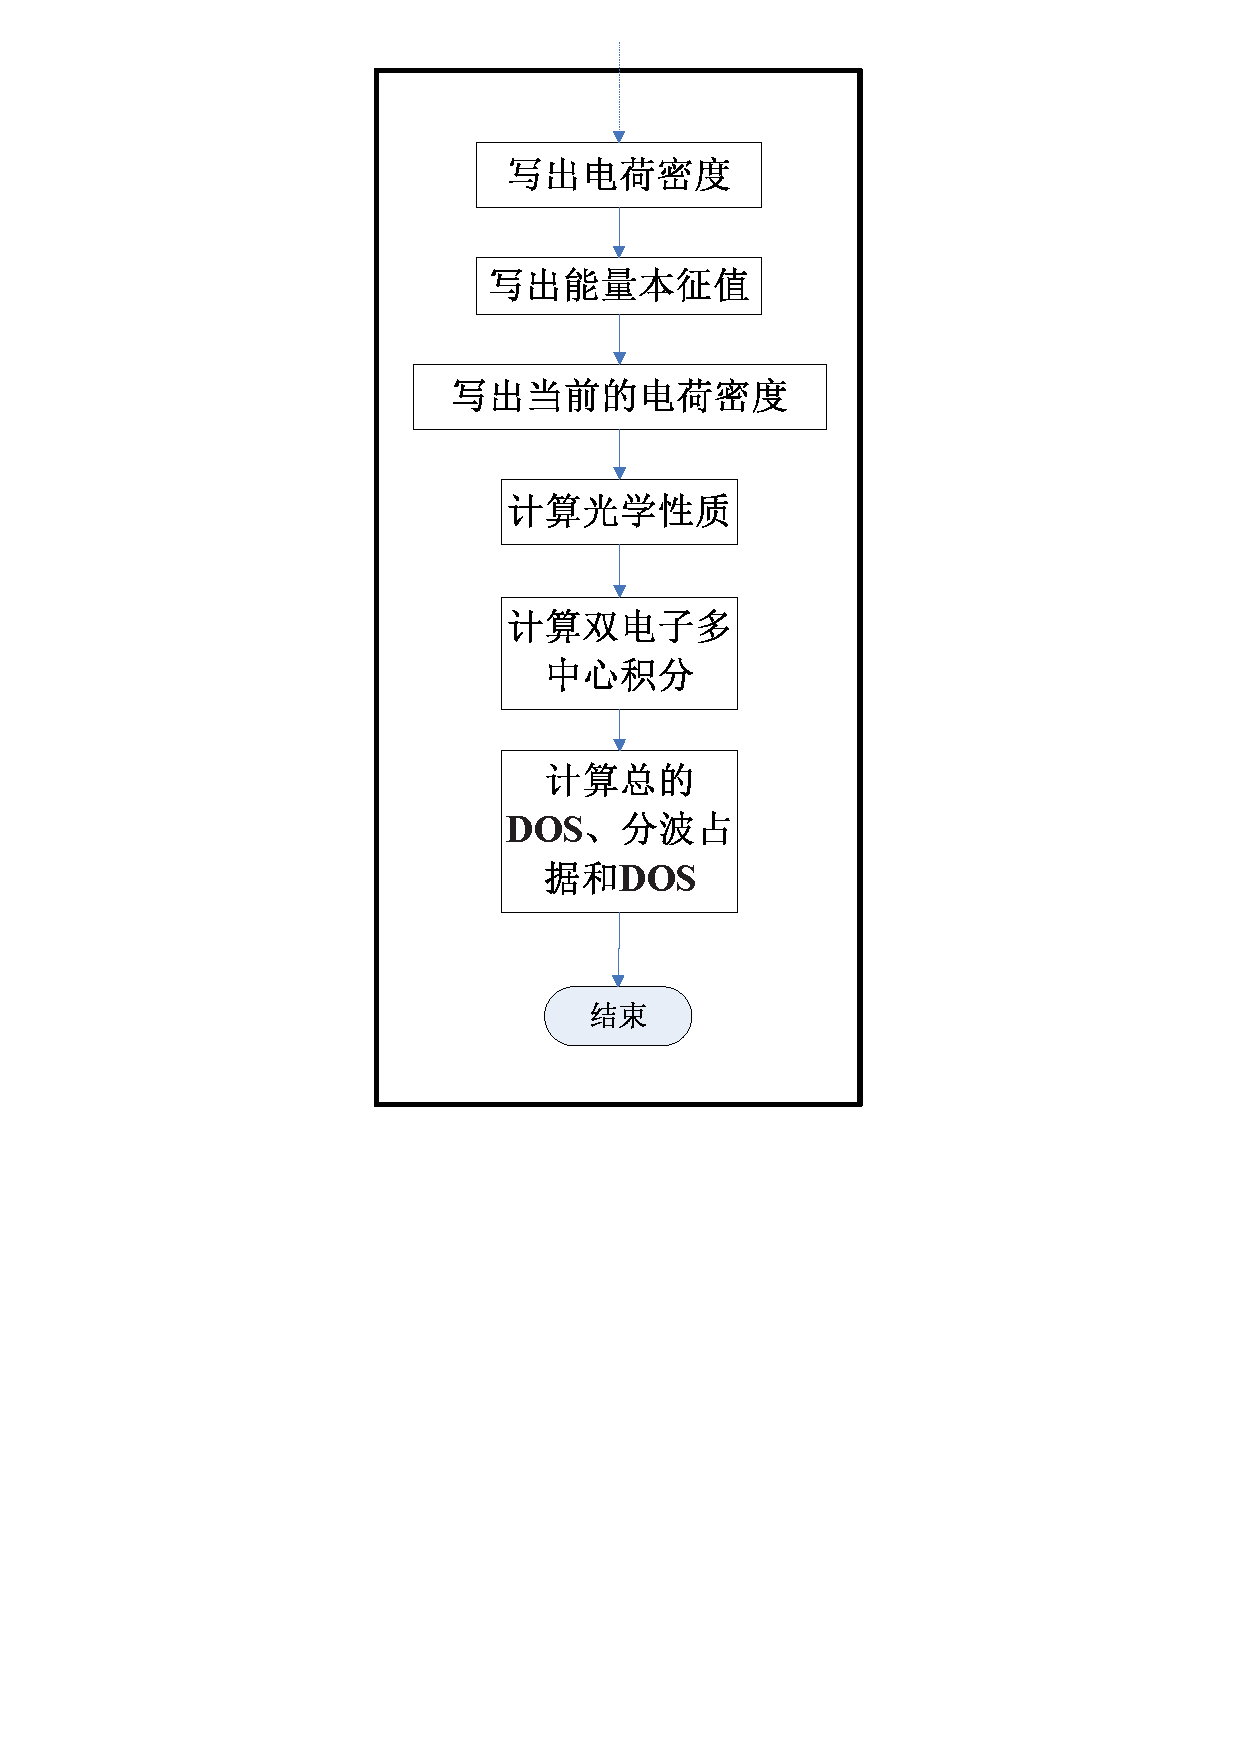
\includegraphics[height=2.30in,width=4.0in,viewport=0 215 562 530,clip]{Figures/VASP_main_Flow-4.png}
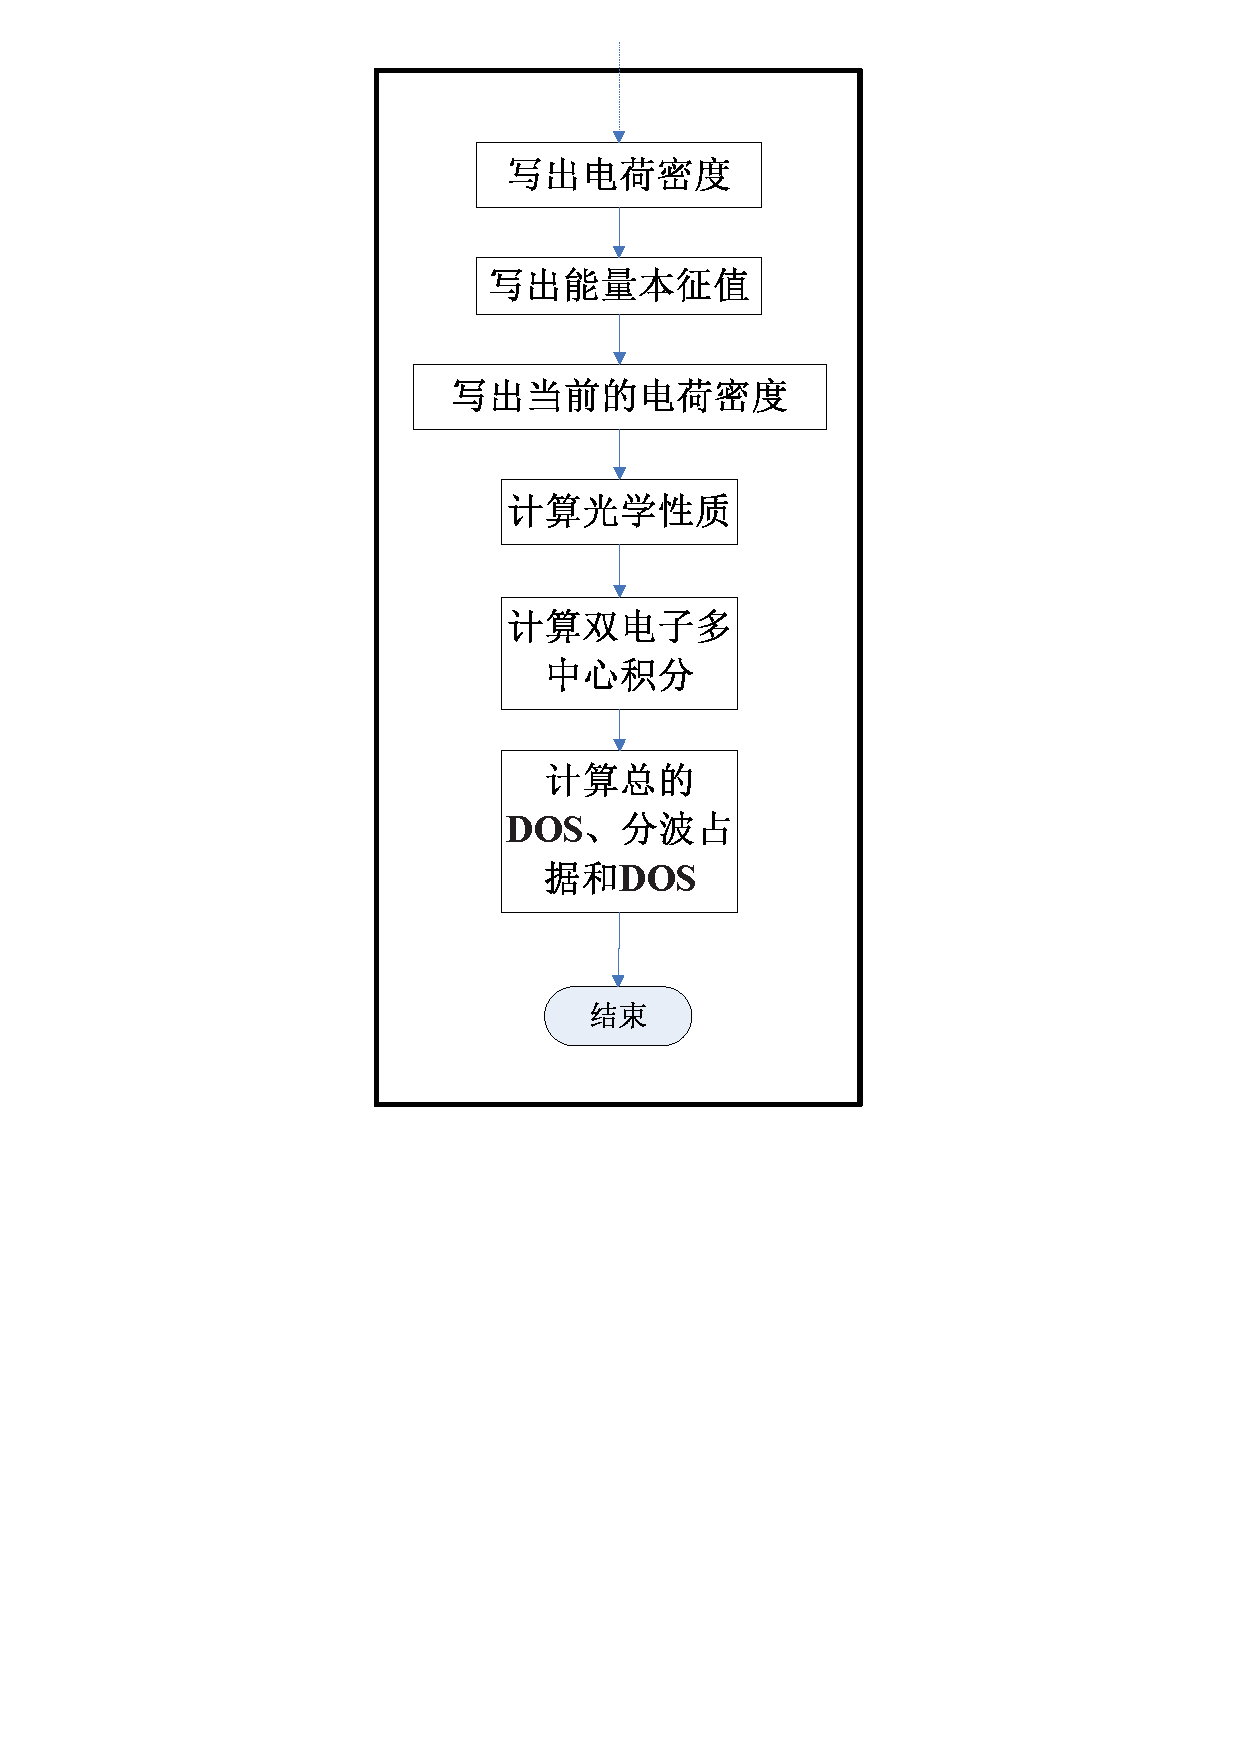
\includegraphics[height=1.40in,width=4.0in,viewport=0 0 562 215,clip]{Figures/VASP_main_Flow-4.png}
\caption{\tiny \textrm{The Flow of main program for VASP.}}%(与文献\cite{EPJB33-47_2003}图1对比)
\label{FLOW_of_VASP}
\end{figure}
\end{frame}

\frame
{
	\frametitle{\textrm{VASP}的迭代收敛}
	完整的\textrm{VASP}计算流程是离子-电子的耦合自洽迭代,称为从头算分子动力学\textrm{(Ab Initio Molecular Dynamics, AIMD)}\upcite{PRL55-2471_1985,PRB47-10142_1993}
\vskip 3pt
	{\fontsize{6.2pt}{4.2pt}\selectfont{
		\begin{itemize}
		\item \textrm{AIMD}通过在动力学系统中引入经典力学的绝热能量,将\textrm{DFT}与\textrm{MD}关联起来,实现电子与离子运动在同一动力学框架内处理,同时又在时间尺度上保持分离
		\item \textrm{AIMD}框架下,\textrm{DFT}到\textrm{MD}跨尺度无需再借助势函数模拟,电子弛豫过程与分子动力学可以用类似的迭代方式计算,大大降低了程序的复杂度
	\end{itemize} }}
\begin{figure}[h!]
	\vspace{-0.2in}
\centering
%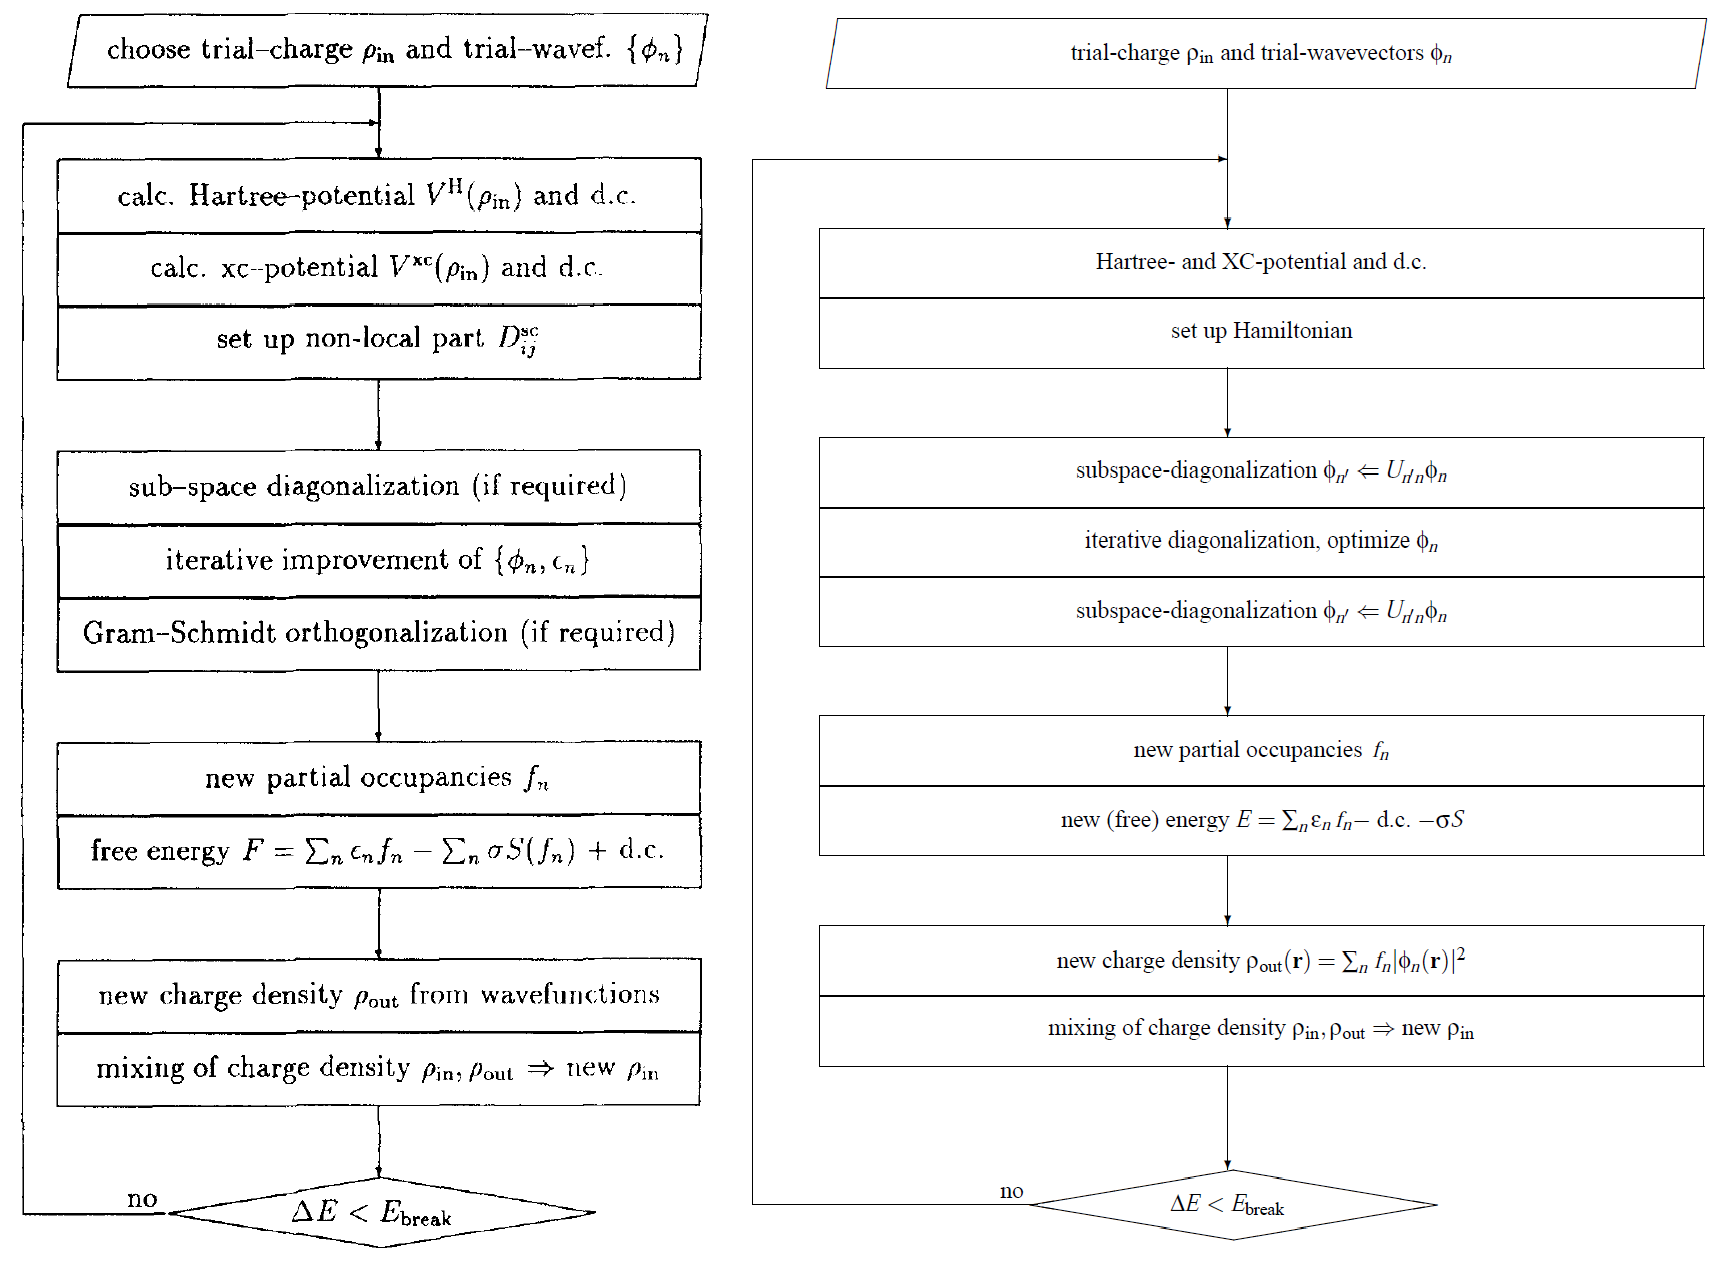
\includegraphics[height=2.7in,width=4.0in,viewport=0 0 1300 960,clip]{Figures/VASP_procedure-full.png}
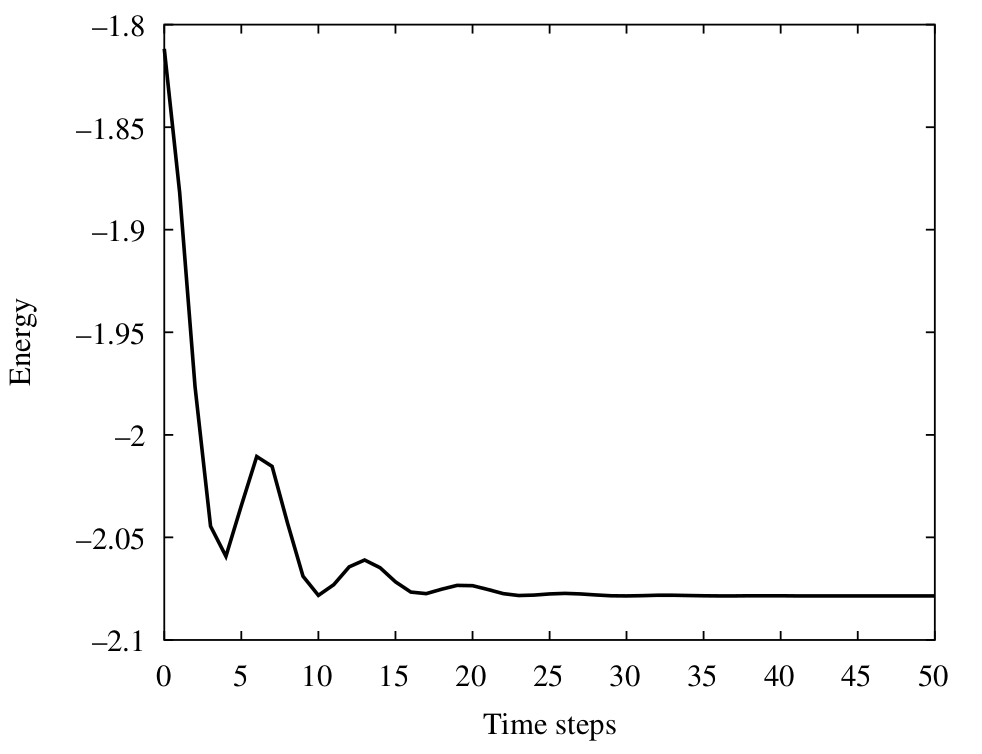
\includegraphics[height=1.8in,width=2.6in,viewport=0 0 740 600,clip]{Figures/Ab-initio-Ene.png}
\caption{\tiny \textrm{The Flow of calculation for the AIMD.}}%(与文献\cite{EPJB33-47_2003}图1对比)
\label{PAW_AIMD}
\end{figure} 
}

\subsection{\rm{VASP}软件概要}
\frame
{
	\frametitle{\textrm{VASP}软件概要}
	作为第一性原理计算的商用软件,\textrm{VASP}已成为计算材料学领域应用最广泛的软件之一。全球绝大多数超算中心都安装了\textrm{VASP},据统计,\textrm{VASP}软件的作业机时占用全球总机时的12$\sim$20\%,但由于其%类似于linpack软件,
属于重型浮点计算密集型应用,实际耗电量占比则高达30$\sim$50\%
\vskip 3pt
	{\fontsize{9.0pt}{7.2pt}\selectfont{
	\begin{itemize}
		\item \textcolor{blue}{物理上},\textrm{VASP}基于\textrm{DFT}近似,求解\textrm{Kohn-Sham}方程,并将粒子基态密度问题转化为矩阵的本征函数和本征值问题
		\item \textcolor{blue}{数学上},方程求解过程的核心是矩阵对角化与\textrm{PDE}的自洽迭代,即便对于简单体系,也需要完成数十次的迭代,而规模大的计算模拟体系则可能需要成千上万次迭代计算
		\item \textcolor{blue}{计算过程上},\textrm{VASP}计算的时长开销主要是本征值求解的矩阵对角化;此外由于算法限制,\textrm{Kohn-Sham}方程作为线性方程组作并行处理时,节点间存在密集的通信。在上千节点,上万计算核的大规模并行系统上,数据通信将严重影响程序的性能,这是当前\textrm{VASP}软件的主要瓶颈
	\end{itemize}}}
			\textcolor{magenta}{有必要探索新的并行和优化策略来提升\textrm{VASP}的计算性能}
}

%------------------------------------------------------------------------Reference----------------------------------------------------------------------------------------------
		\frame[allowframebreaks]
{
\frametitle{主要参考文献}
\begin{thebibliography}{99}
{\tiny
	\bibitem{Crelle30-51_1846}\textrm{C. G. Jacobi,\textbf{\"Uber ein leichtes Verfahren die in der Theorie der S\"acul\"arst\"orrungen vorkommenden Gleichungen numerisch aufzul\"osen}, \textit{Crelle's J.} \textbf{30} (1846), 51-94}
	\bibitem{PRB50-17953_1994}\textrm{P. E. Bl\"ochl. \textit{Phys. Rev.} B, \textbf{50} (1994), 17953}
	\bibitem{PRB59-1758_1999}\textrm{G. Kresse and D. Joubert \textit{Phys. Rev.} B, \textbf{59} (1999), 1758}
	\bibitem{PRL55-2471_1985}\textrm{R. Car and M. Parrinello \textit{Phys. Rev.} Lett., \textbf{55} (1985), 2471}
	\bibitem{PRB47-10142_1993}\textrm{K. Laasonen and A. Pasquarello and R. Car and C. Lee and D. Vanderbilt \textit{Phys. Rev.} B, \textbf{47} (1993), 10142}
	\bibitem{Elect_Stru}\textrm{Richard. M. Martin. \textit{Electronic Structure: Basic Theory and Practical Methods} (Cambridge University Press, Cambridge, England, 2004)}
        \bibitem{Singh}\textrm{D. J. Singh. \textit{Plane Wave, PseudoPotential and the LAPW method} (Kluwer Academic, Boston,USA, 1994)}					%
}
\end{thebibliography}
%\nocite*{}
}
%-----------------------------------------------------------------------------------------------------------------------------------------------------------------------%
